\documentclass[12pt]{report}

\usepackage[titletoc]{appendix}
\usepackage{datetime}
\usepackage{graphicx}
\usepackage{amsmath}
\usepackage{algorithmicx}
\usepackage{algorithm}
\usepackage[explicit]{titlesec}
\usepackage{tocloft}
\usepackage{amssymb}
\usepackage{longtable}
\usepackage{multirow}
\usepackage[english]{babel}

\usepackage{subcaption}
\usepackage{subfig}

\usepackage{url}

\usepackage{rotating}

\usepackage{varwidth}
\usepackage{setspace}
\usepackage{perpage}
\usepackage{enumerate}
\MakePerPage{footnote}

\usepackage{tikz}
\usetikzlibrary{arrows,positioning,automata}
\usepackage[noend]{algpseudocode}

\usepackage{mathtools}

\usepackage{caption}

\renewcommand{\familydefault}{\rmdefault}
\renewcommand\cftchapaftersnum{.}
\renewcommand\cftchapdotsep{\cftdotsep}

\setlength{\textheight}{8.63in}
\setlength{\textwidth}{5.9in}
\setlength{\topmargin}{-0.2in}
\setlength{\oddsidemargin}{0.3in}
\setlength{\evensidemargin}{0.3in}
\setlength{\headsep}{0.0in}

\titleformat{\chapter}[block]
  {\Large\filcenter\bfseries}{\MakeUppercase{Chapter \thechapter}\\}{0em}{\MakeUppercase{#1}}
  
\titleformat{\section}[block]
  {\large\bfseries}{\thesection}{0.5em}{#1}
  
\titleformat{\subsection}[block]
  {\normalsize\bfseries}{\thesubsection}{0.5em}{#1}
  

\newcommand{\signature}{\rule{3in}{1.2pt}}
\newcommand{\thesistitle}{Affective Motivational Collaboration Theory}
\newdateformat{monthyear}{\monthname[\THEMONTH] \THEYEAR}

\DeclareMathOperator*{\argmin}{\arg\!\min}
\DeclareMathOperator*{\argmax}{\arg\!\max}

\linespread{1.5}

\begin{document}

\begin{titlepage}
\begin{center}
\large\textbf{\thesistitle}\\[0.5em]

\large\textnormal{by}\\
\large\textnormal{Mahni Shayganfar - mshayganfar@wpi.edu}\\[0.5em]

\large\textnormal{A PhD Dissertation}\\[0.5em]

\large\textnormal{Presented at}\\[0.5em]
\large\textsc{WORCESTER POLYTECHNIC INSTITUTE}\\[0.5em]
\large\textnormal{in partial fulfillment of the requirements for the}\\[0.5em]
\large\textnormal{DOCTOR OF PHILOSOPHY}\\[0.5em]
\large\textnormal{in}\\
\large\textnormal{Computer Science}\\
\large\textnormal{November 2016}\\[0.75em]
\end{center}

\noindent\large\textsc{Approved}\\[0.5em]
\Large\textnormal{\signature}\\
\normalsize\textnormal{Professor Charles Rich, Thesis Advisor}\\[0.5em]
\Large\textnormal{\signature}\\
\normalsize\textnormal{Professor Candace L. Sidner, Thesis Co-Advisor}\\[0.5em]
\Large\textnormal{\signature}\\
\normalsize\textnormal{Professor John E. Laird, Thesis Committee
Member}\\[0.5em] \Large\textnormal{\signature}\\
\normalsize\textnormal{Professor Stacy Marsella, Thesis Committee Member}
\end{titlepage}

\thispagestyle{empty}
\vspace*{\fill}
  \begin{center}
    \textcopyright \hspace{0.5em} Copyright by Mahni Shayganfar 2016

    All Rights Reserved
  \end{center}
\vspace*{\fill}
\newpage

\pagenumbering{roman}

\chapter*{Abstract}
\addcontentsline{toc}{chapter}{Abstract}

Abstract Here!

\pagebreak

\chapter*{Acknowledgments}
\addcontentsline{toc}{chapter}{Acknowledgments}

Acknowledgments Here!

\pagebreak

\tableofcontents
\pagebreak

\listoffigures
\pagebreak

\listoftables
\pagebreak

%\listofalgorithms
%\addcontentsline{toc}{chapter}{List of Algorithms}
%\pagebreak

\pagenumbering{arabic}

\chapter{Introduction}
\label{ch:introduction}

\section{Motivation}

The idea of robots or other intelligent agents living in a human environment has
been a persistent dream from science fiction books to artificial intelligence
and robotic laboratories. Collaborative robots are expected to become an
integral part of humans' environment to accomplish their industrial and
household tasks. In these environments, humans will be involved in robots'
operations and decision-making processes. The involvement of humans influences
the efficiency of robots' interaction and performance, and makes the robots
sensitive to humans' cognitive abilities and behaviors.

A key aspect of the sociability of robots is their ability to collaborate with
humans in the same environment. Collaboration is a coordinated activity in which
the participants work jointly to satisfy a shared goal
\cite{grosz:plans-discourse}. There are many challenges in achieving a
successful collaboration between robots and humans. To meet these challenges, it
is crucial to understand what makes a collaboration not only successful, but
also efficient. Existing computational models of collaboration explain some of
the important concepts underlying collaboration; such as the presence of a
reason for collaborators' commitment, and the necessity of communicating about
mental states in order to maintain progress over the course of a collaboration.
The most prominent collaboration theories are based on plans and intentions
\cite{cohen:teamwork} \cite{grosz:plans-discourse}
\cite{Litman:discourse-commonsense}, and are derived from Bratman's BDI
architecture \cite{bratman:intentions-plans}. Two theories, Joint Intentions
\cite{cohen:teamwork} and SharedPlans
\cite{grosz:planning-acting,grosz:collaboration,grosz:plans-discourse}, have
been used to support teamwork and collaboration between humans and robots or
virtual agents \cite{breazeal:humanoid-robots}
\cite{montreuil:planning-robot-activity} \cite{sidner:enagagement-robot}
\cite{yen:cast}. However, these theories explain only the structure of a
collaboration. For instance, in SharedPlans theory collaborators build a shared
plan containing a collection of beliefs and intentions about the actions in the
plan. Collaborators communicate these beliefs and intentions via utterances
about actions that contribute to the shared plan. This communication leads to
the incremental construction of a shared plan, and ultimately successful
completion of the collaboration. In contrast, in Joint Intentions theory, the
notion of joint intention is viewed as a persistent commitment of the team
members to a shared goal. In this theory, once an agent enters into a joint
commitment with other agents, it should communicate its private beliefs to other
team members.

Although existing collaboration theories explain the important elements of a
collaboration structure, the underlying processes required to dynamically
create, use, and maintain the elements of this structure are largely
unexplained. For instance, a general mechanism has yet to be developed that
allows an agent to effectively integrate the influence of its collaborator's
perceived or anticipated emotions into its own cognitive mechanisms to prevent
shared task failures while maintaining collaborative behavior. Therefore, a
process view of collaboration must include certain key elements. It should
inherently involve social interactions since all collaborations occur between
social agents, and it should essentially constitute a means of modifying the
content of social interaction as the collaboration unfolds. The underlying
processes of emotions possess these two properties, and social functions of
emotions explain some aspects of the underlying processes in collaboration. This
thesis makes the case for emotion-driven processes within collaboration and
demonstrates how it furthers collaboration between humans and robots.

\section{Thesis Statement and Scope}

In this thesis, we develop and validate a framework based on \textit{Affective
Motivational Collaboration Theory} which can improve the effectiveness of
collaboration between agents/robots and humans. This thesis is established based
on the reciprocal influence of collaboration structure and the appraisal
processes in a dyadic collaboration. We focus only on two-participant
collaboration; teamwork collaboration is out of our scope. Furthermore, this
work focuses on a) the influence of emotion-regulated processes on the
collaboration structure, and b) prediction of the observable behaviors of the
other during a collaborative interaction.

We describe the cognitive processes involved in a collaboration in the context
of a cognitive architecture. There are several well-developed cognitive
architectures, e.g., Soar \cite{laird:soar} and ACT-R \cite{anderson:act-r},
each with different approaches to defining the basic cognitive and perceptual
operations. There have also been efforts to integrate affect into these
architectures \cite{dancy:actR-physiology-affect, marinier:behavior-emotion}. In
general, however, these cognitive architectures do not focus on processes to
specifically produce emotion-regulated goal-driven collaborative behaviors. At
the same time, existing collaboration theories, e.g., SharedPlans
\cite{grosz:plans-discourse} theory, focus on describing the structure of a
collaboration in terms of fundamental mental states, e.g., mutual beliefs or
joint intentions. However, they do not describe the associated processes, their
relationships, and influences on each other. \textit{Affective Motivational
Collaboration Theory} deals with some of the major affect-driven processes
having an impact on the collaboration structure. This theory is informed by
research in psychology and artificial intelligence which is reviewed in Chapter
\ref{ch:background}. Our contribution, generally speaking, is to synthesize
prior work on appraisal and collaboration, and motivation to provide a new
theory which describes some of the prominent emotion-regulated goal-driven
phenomena in a dyadic collaboration.

\section{Contributions}

Throughout this work we aim to show how a robot can leverage emotion-driven
processes using appraisal algorithms to improve collaboration with humans. As
such, in this thesis work, we introduce a novel framework, called Affective
Motivational Collaboration (AMC) framework, which allows a robotic agent to
collaborate with a human while incoporating the underlying emotion-driven
processes and the expressed emotion of the human collaborator. Such a framework
is built based on computational models of collaboration and appraisal allowing
for task-driven interaction with robots or other agents. The theoretical
foundation, computational models and algorithms as well as the overall
framework, and the end-to-end evaluation of the framework make the following
contributions:

\begin{enumerate}
  \item \textbf{Introducing \textit{Affective Motivational Collaboration Theory}:}
    
  	(Chapter \ref{ch:amct}) As mentioned earlier, since the theoretical
  	foundation of AMC framework is built on the combination of SharedPlans
  	theory of collaboration \cite{grosz:plans-discourse} and cognitive appraisal
  	theory of emotions \cite{marsella:ema-process-model}
  	\cite{scherer:appraisal-processes}, one of the contributions of our work is
  	to introduce theoretical concepts incorporating key notions of both theories
  	in a dyadic collaboration context. Applying cognitive appraisal theory in the
  	collaboration context is novel. Other models of the appraisal theory have not
  	paid attention to the dynamics of the collaboration.
	
  \item \textbf{Developing new computational models and algorithms for
  \textit{Affective Motivational Collaboration Framework}:}
  
	(Chapter \ref{ch:appraisals}) Another contribution of our work is to create
	computational models and algorithms to compute the value of appraisal variables
	in a dyadic collaboration. We use the collaboration structure to compute
	appraisal variables. Reciprocally, we use the evaluative nature of the
	appraisal to make changes to the collaboration structure as required. We have
	also developed a new algorithm for emotion-driven goal management in the
	context of collaboration. Goal management is one of the important functions of
	emotions during collaboration. Existing models and implementations of emotions
	focus only on how emotions regulate and control internal processes and
	sometimes behaviors. This part of our work shows how appraisal components of
	the self and the human collaborator contributes to goal management as an
	emotion function.
  
  \begin{figure*}
    \centering
    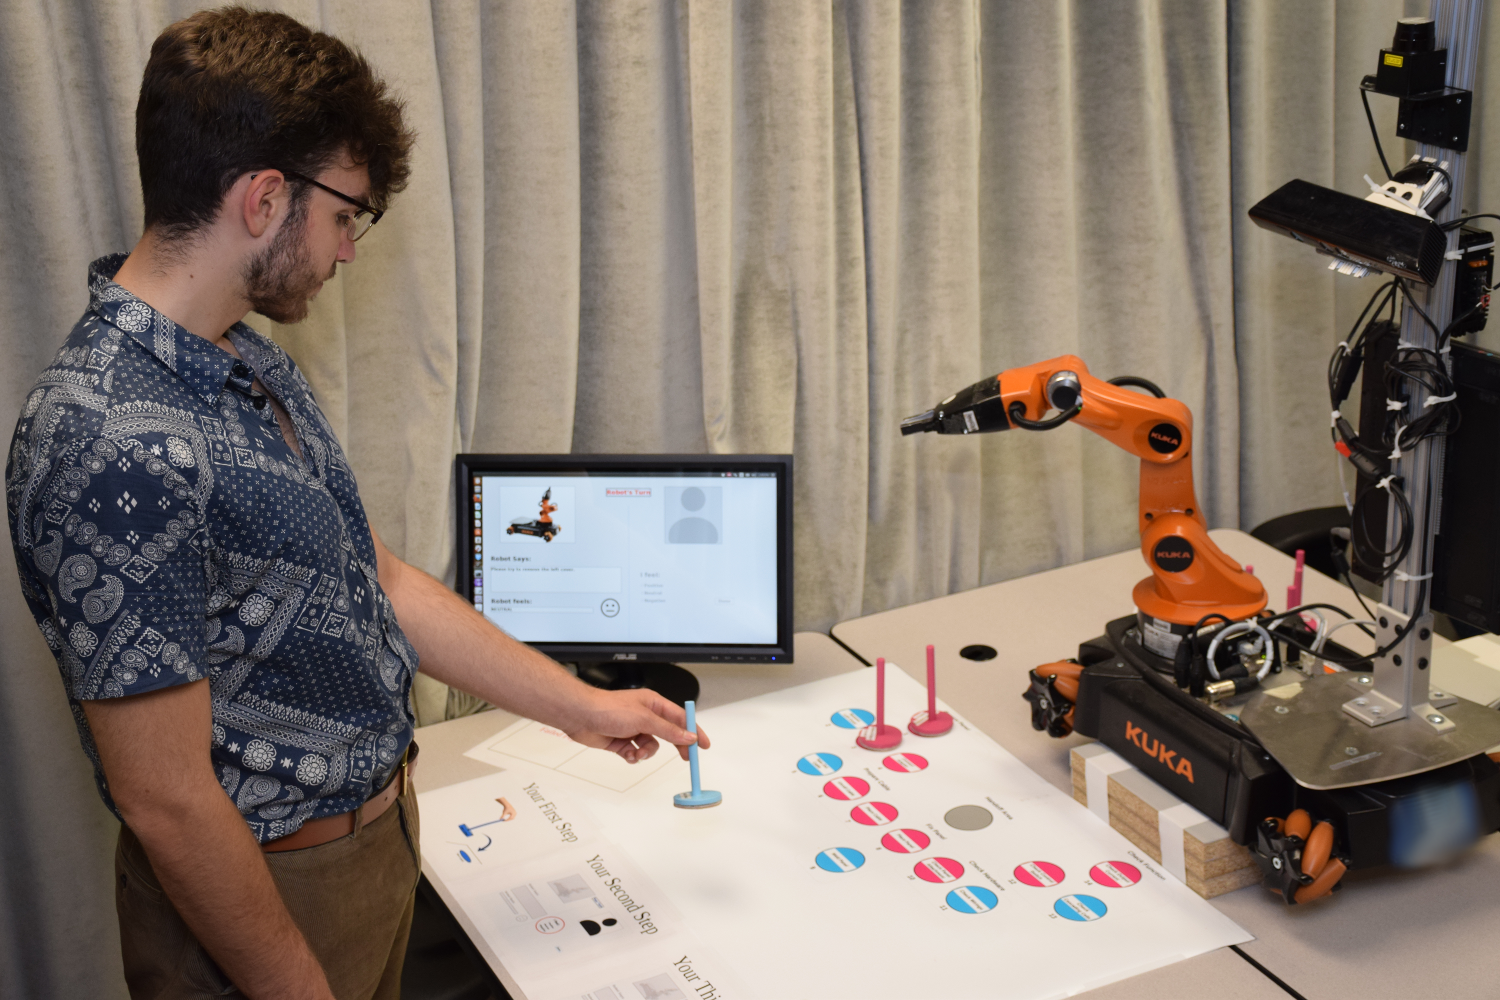
\includegraphics[scale=1.17]{figure/collaborative-robot.png}
    \caption{A robotic arm collaborating with a human to achieve a shared goal
    using \textit{Affective Motivational Collaboration Framework}.}
    \label{fig:collaborative-robot}
  \end{figure*}
  
  \item \textbf{Developing a computational framework based on \textit{Affective
  Motivational Collaboration Theory}:}

  (Chapter \ref{ch:framework}) In order to evaluate our computational models and
  algorithms within an interaction with human collaborators, we have developed
  a computational framework based on our theoretical foundations in
  \textit{Affective Motivational Collaboration Theory}. Our computational
  framework implements the key concepts related to \textit{Affective
  Motivational Collaboration Theory} as well as minimal implementation of other
  processes which are required for validation of the model but are not part of
  this thesis' contributions. The emphasis of the model is on the underlying
  cognitive processes of collaboration and appraisal concepts, rather than the
  Perception and the Action mechanisms.

  \item \textbf{Validating \textit{Affective Motivational Collaboration
  Theory:}}

  (Chapters \ref{ch:appraisals} and \ref{ch:awareness}) We have conducted two
  user studies a) to validate our appraisal algorithms before further
  development of our framework, and b) to investigate the overall functionality
  of our framework within an end-to-end system evaluation with participants
  and a robot. The second user study was also conducted to evaluate the benefit
  of using our computational framework in human-robot collaboration. In the
  first user study, we crowd sourced our questionnaires to test our hypothesis
  that humans and our algorithms will provide similar answers to questions
  related to different factors within our appraisal algorithms. In the second
  user study, we investigated the importance of emotional awareness in
  human-robot collaboration, and the overall functionality of the AMC framework
  with the participants in our study environment.
\end{enumerate}

\chapter{Background and Related Work}
\label{ch:background}

\section{Computational Collaboration Theories}

\subsection{Shared-Plans Theory}

\subsection{Joint-Intentions Theory}

\subsection{Hybrid Theories}

\subsection{Similarities and Differences}

\subsection{Applications of Collaboration Theories}

\section{Affective Computing}

\subsection{Affect and Emotions}

\subsection{Functions of Emotions}

\subsection{Motivation and Theory of Mind}

\section{Computational Models of Emotions}

\subsection{Appraisal Theory}

\subsection{Other Computational Models}

\subsection{Similarities and Differences}

\subsection{Applications in Autonomous Agents and Robots}

\chapter{Affective Motivational Collaboration Theory}
\label{ch:amct}

\section{Introduction}
Current computational theories used for human-robot collaboration specify the
structure of collaborative activities, but are weak on the underlying processes
that generate and maintain these structures. We argue that emotions are crucial
to these underlying processes and we have developed a new computational theory,
called Affective Motivational Collaboration Theory, that combines emotion-based
processes, such as appraisal and coping, with collaboration processes, such as
planning, in a single unified framework. This work is implemented as part of a
larger effort to build robots capable of generating and recognizing emotions in
order to be better collaborators. We have investigated the mutual influences of
affective and collaborative processes in a cognitive theory to support
interaction between humans and robots or virtual agents. We build primarily on
the \textit{cognitive appraisal} theory of emotions and the \textit{SharedPlans}
theory of collaboration to investigate the structure, fundamental processes and
functions of emotions in a collaboration. We have developed new algorithms for
appraisal processes as part of a new overall computational model. We have
evaluated our implemented appraisal algorithms by conducting an online user
study.

Although existing collaboration theories explain the important elements of a
collaboration structure, the underlying processes required to dynamically
create, use, and maintain the elements of this structure are largely
unexplained. For instance, a general mechanism has yet to be developed that
allows an agent to effectively integrate the influence of its collaborator's
perceived or anticipated emotions into its own cognitive mechanisms to prevent
shared task failures while maintaining collaborative behavior. Therefore, a
process view of collaboration must include certain key elements. It should
inherently involve social interactions since all collaborations occur between
social agents, and it should essentially constitute a means of modifying the
content of social interaction as the collaboration unfolds. The underlying
processes of emotions possess these two properties, and social functions of
emotions explain some aspects of the underlying processes in collaboration.
This work is implemented as part of a larger effort to build robots capable of
generating and recognizing emotions in order to be better collaborators.

There is also a communicative aspect of emotions. For instance, emotions are
often intended to convey information to others \cite{goffman:self-presentation}.
Emotions are also involved in verbal behaviors. For instance, an utterance can
include both content and relational meaning. An emotion might appear to be
elicited by the content of the utterance, but in fact be an individual's
response to the relational meaning \cite{planalp:communicating-emotion}. The
interpretation of these relational meanings are handled by the appraisal of
events. Appraisal processes give us a way to view emotion as social
\cite{hooft:sharing-emotions}. Meaning is created by an individual's social
experiences in the social world, and individuals communicate these meanings
through utterances. Consequently, the meaning of these utterances and the
emotional communication change the dynamic of social interactions. A successful
and effective emotional communication necessitates ongoing reciprocal
adjustments between interactants that can happen based on interpretation of each
other's behaviors \cite{parkinson:emotion-social-interaction}. This adjustment
procedure requires a baseline and an assessment procedure. While the components
of the collaboration structure, e.g., shared plan, provide the baseline,
emotion-related processes (e.g., appraisal) provide the assessment procedure.

\subsection{Scenario}

\subsection{Example of a Collaborative Interaction}

\section{Design and Architecture}

\subsection{Mechanisms}

\subsection{Functions of Emotions}

\subsection{Mental States}
\label{sec:mental-states}

\subsection{Attributes of Mental States}

\chapter{Computational Framework}
\label{ch:appraisals}

\vspace*{-2mm}
\section{Introduction}
\vspace*{-3mm}
In this chapter, we focus on the specific problem of appraising the
\textit{Relevance} (since other appraisals are only computed for relevant
events), \textit{Desirability} (since it discriminates facilitating and
inhibitory events towards the collaboration progress), \textit{Expectedness}
(since it underlies a collaborative robot's attention), and
\textit{Controllability} (since it is associated with the agent's coping
ability) of events within a collaborative interaction. Our contribution is to
ground general appraisal concepts in the specific context and structure of
collaboration.

There are several appraisal models (e.g., EMA \cite{marsella:ema-process-model})
contributing in different applications such as social sciences, virtual agents,
and robotics. However, none of these models have focused on the appraisal
processes during collaboration. We believe appraisal plays a key role in
collaboration due to its regulatory and evaluative nature. Also, collaboration
induces some changes to appraisal processes due to its unique nature. For
instance, although the appraisal models mostly use utility to compute the
relevance of an event, we have found new cognitive components involved in
determining utility because of the influence of the collaboration. These
components, such as the recurrence of a belief by the human collaborator or the
influence of the human collaborator's perceived emotion on the robot's decisions
emphasize the fact that collaboration requires different procedures in appraisal
processes.

\vspace*{-5mm}
\section{Collaboration Mechanism}
\vspace*{-4mm}
The collaboration and Appraisal mechanisms have reciprocal influence on each
other. In this section, we focus on information about collaboration structure
which will be incorporated in appraisal processes in Section
\ref{sec:appraisal}. We describe some of the methods in our Collaboration
mechanism which are used to retrieve information about the collaboration
structure.

The Collaboration mechanism constructs a hierarchy of goals associated with
tasks in the form of a hierarchical task network (see Figure \ref{fig:cs}), and
also manages and maintains the constraints and other required details of the
collaboration including the inputs and outputs of individual tasks, the
\textit{preconditions} (specifying whether it is appropriate to perform a task),
and the \textit{postconditions} (specifying whether a just-completed task was
successful). Collaboration also keeps track of the focus of attention, which
determines the salient objects, properties and relations at each point, and
shifts the focus of attention during the interaction.

\begin{figure}[t]
  \centering
  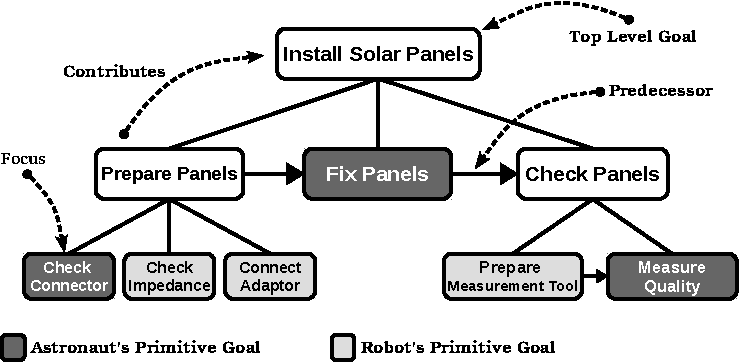
\includegraphics[width=0.97\textwidth]{figure/collaborationStructure-small-croped.pdf}
  \caption{{\fontsize{10}{10}\selectfont Collaboration structure (shared
  plan).}}
  \label{fig:cs}
  \vspace*{-5mm}
\end{figure}

Here, we describe the methods which retrieve information about the collaboration
structure, and are used in our algorithms to compute the values of appraisal
variables. In these methods, $\varepsilon_t$ is the event corresponding to time
\textit{t}, and $g_t$ is a given goal at time \textit{t}.

\begin{itemize}
  \setlength\itemsep{1mm}
  \item \textit{recognizeGoal($\varepsilon_t$)} returns the unique goal to which
  the given event (action, utterance, or emotional expression) directly
  contributes; it is only one goal since the robot can only do one primitive
  action at a time in our collaboration model, i.e, in the goal tree, a given
  primitive action can only directly contribute to one parent goal. The method
  returns \textit{ambiguous} if it does not recognize a goal in the
  plan\footnote{Ambiguity introduces some extra complexities which are beyond
  scope of this paper.}.
  
  \item \textit{getGoalStatus($g_t$)} returns whether $g_t$'s status is
  \textsc{achieved, failed, blocked, inapplicable, pending,} or \textsc{in
  progress}. In our example, ``Check Connector'' is the current (focused) goal
  and it is \textsc{pending}, and the ``Prepare Panels'' and ``Install Solar
  Panels'' are \textsc{in progress}. The focused goal is the goal that the robot
  currently pursues.
  
  \item \textit{getTopLevelGoal($g_t$)} returns $g_t$'s top level goal.

  \item \textit{precondStatus($g_t$)} returns the status of the precondition for
  the given goal whether it is \textsc{satisfied, unsatisfied} or
  \textsc{unknown}. For instance, the precondition for fixing a panel is whether
  the panel is appropriately located on its frame.
  
  \item \textit{isLive($g_t$)} returns \textit{true} if all the predecessors of
  $g_t$ are \textsc{achieved} and all the preconditions are \textsc{satisfied},
  i.e., \textsc{pending} or \textsc{in progress} goals; otherwise returns
  \textit{false}.
  
  \item \textit{isFocusShift($g_t$)} returns \textit{true} if the given
  goal is not the previous focus (top of the stack); otherwise returns
  \textit{false}.
  
  \item \textit{isNecessaryFocusShift($g_t$)} returns \textit{true} if the
  status of the previous focus was \textsc{achieved}; otherwise returns
  \textit{false} \cite{rich:focused-unfocused-users}.
  
  \item \textit{isPath($g_1$, $g_2$)} returns \textit{true} if there is a path
  between $g_1$ and $g_2$ in a plan tree structure; otherwise returns
  \textit{false}.
  
%   \item \textit{doesContribute($g_t$)} returns whether the given goal
%   contributes to another goal in the higher level of the plan hierarchy. For
%   instance, an abstract (nonprimitive) goal of ``Bring Panels'' contributes to
%   the higher level goal of ``Install Solar Panels''.
  
  \item \textit{getContributingGoals($g_t$)} returns $g_t$'s children.
  
  \item \textit{getPredecessors($g_t$)} returns $g_t$'s predecessors.
  
  \item \textit{getInputs($g_t$)} returns all required inputs for $g_t$. For
  example, the goal ``Fix Panels'' requires inputs such as \textit{welding tool}
  and \textit{panel}.
  
  \item \textit{isAvailable($g_t$)} returns whether the given input is
  available. For instance, whether the \textit{welding tool} is available for the
  goal ``Fix Panels''.
  
%   \item \textit{isAchieved($g_t$)} returns whether the given goal is achieved,
%   i.e., whether all the postconditions of the given goal are \textsc{satisfied}.
  
  \item \textit{isFocused($g_t$)} returns whether the focus is on $g_t$.
  
  \item \textit{getResponsible($g_t$)} returns responsible agent(s) for $g_t$.
  In a dyadic collaboration, both of the agents (jointly) can be partly
  responsible for a nonprimitive goal, while each (self or other) is responsible
  for one or more primitive goals. For instance, both the Robot and the
  Astronaut are responsible for the nonprimitive goal of ``Install Solar
  Panels'', whereas it is only the Robot who is responsible for the
  primitive goal of ``Prepare Measurement Tool''.
\end{itemize}

\section{Appraisal Mechanism and Underlying Processes}
\label{sec:appraisal}
As we mentioned earlier, we consider four appraisal variables to be the most
important appraisal variables in a collaboration context, i.e., Relevance,
Desirability, Expectedness, and Controllability. There are other appraisal
variables introduced in psychological \cite{scherer:appraisal-processes} and
computational literature \cite{gratch:domain-independent}. We believe most of
these variables can be straightforwardly added to our appraisal mechanism
whenever they are required. All of the algorithms in this section use mental
states of the robot (discussed in Section \ref{sec:mental-states}) which are
formed based on the collaboration structure (Figure
\ref{fig:appraisal-collaboration}). These algorithms use the corresponding
recognized goal of the most recent event at each turn.

\begin{figure}[tbh]
  \centering
  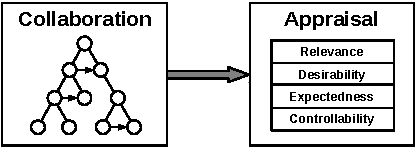
\includegraphics[width=0.8\textwidth]{figure/appraisal-collaboration-croped.pdf}
  \caption{Using Collaboration structure in Appraisal (mechanisms in our
  framework).}
  \label{fig:appraisal-collaboration}
\end{figure}

\subsection{Relevance}
Relevance is an important appraisal variable since the other appraisal variables
are meaningful only for relevant events. Relevance as an appraisal variable
measures the significance of an event for the self. An event can be evaluated to
be relevant if it has a non-zero utility \cite{marsella:ema-process-model}.
However, the utility of an event is also influenced by the other collaborator's
emotional expressions as the reflection of the other collaborator's mental state
with respect to the status of the collaborative environment. Other appraisal
models only consider the utility of an event based on the self's goal and plan.

Algorithm \ref{alg:relevance} determines the relevance of the given event with
respect to the current mental state. The relevance of the event depends on the
significance of the event with respect to the collaboration status, which is
determined based on the utility of the event as presented in
\cite{gratch:domain-independent,marsella:ema-process-model}. Our algorithm for
computing the relevance of an event during collaboration involves other factors
that other appraisal models do not consider. For instance, the human's
perceived emotion, recurrence of a belief, or occurrence of a belief about an
unrelated goal by the human play important roles by influencing the utility
of an event during collaboration. As a result, evaluating the relevance of
events can cause a collaborative robot to respond effectively which can
positively impact the status of the shared goal, without dedicating all its
resources to every event.

After perceiving an event, the belief about that event represents the event in
the robot's mental state. \textit{recognizeGoal} returns the goal to which the
current event contributes, unless it is \textit{ambiguous}; $g_{t}$ represents
the shared goal at time (turn) $t$ within the shared plan. We compute the
utility ($-1 \leq \mathcal{U} \leq 1$) of the event using the values of the
attributes associated with the existing beliefs, and the attributes of the
motive associated with the recognized goal (see details below). We use three
belief attributes (see Section \ref{sec:mental-states}) to compute the
belief-related part of the utility:

\begin{algorithm}
	\caption{(Relevance)}
	\label{alg:relevance}
	\begin{algorithmic}[1]
		\Function{IsEventRelevant}{Event $\varepsilon_t$}
 			\Statex
			\State $\mathit{g}_{t} \gets \textit{recognizeGoal}{(\varepsilon_t)}$
 			\Statex
			\State $\mathcal{U} \gets \Call{getEventUtility}{\mathit{g}_{t}}$ 
			\State $\tau_{t} \gets \Call{getEmotionalThreshold}{\mathit{g}_{t}}$
 			\Statex
			\If {$(\tau_{t} \leq |\mathcal{U}|)$}  
 				\State \Return {{\fontsize{7}{8}\selectfont RELEVANT}}
			\Else 
 				\State \Return {{\fontsize{7}{8}\selectfont IRRELEVANT}}
			\EndIf
		\EndFunction
	\end{algorithmic}
\end{algorithm}

\begin{itemize}
  \setlength\itemsep{1mm}
  \item \textit{Strength}: The extent to which the preconditions ($\alpha$),
  postconditions ($\beta$), predecessors ($\lambda$), and contributing goals
  ($\mu$) of a goal are known (\textsc{satisfied} or \textsc{unsatisfied}) makes
  beliefs about the goal stronger. An \textsc{unknown} pre and postcondition
  status of a goal and its predecessors and contributing goals forms weaker
  beliefs. For instance, if one knows all predecessors of a pursued goal (e.g.,
  ``Check Panels'') are \textsc{satisfied} (i.e., ``Fix Panels'' and ``Prepare
  Panels''), failure of the pursued goal will elicit one's negative emotion (due
  to the strong beliefs related to the goal); whereas not knowing the status of
  the goal-related factors (e.g., whether the Astronaut could find the tool to
  fix a panel) causes one to form weaker beliefs about the goal.
  \item \textit{Saliency (S)}: Beliefs related to the focused goal are more
  salient than beliefs related to any other goal in the plan; according to
  Figure \ref{fig:cs}, if one of the collaborators is preparing a solar panel,
  beliefs related to all of the other \textit{live} (\textsc{pending} or
  \textsc{in progress}) goals (e.g. ``Connect Adaptor'') will be less salient
  than beliefs related to the focused goal, i.e., ``Check Connector''. Beliefs'
  saliency decreases according to their corresponding \textit{live} goal's
  distance from the focused goal in the shared plan. \textit{Non-live} goals
  will not be salient.
  \item \textit{Persistence (P)}: The recurrence of a belief over time (turns)
  increases the persistence of the belief. Beliefs occurring only once have the
  lowest value of persistence. For instance, if the Astronaut keeps saying that
  she can not find the measurement tool to check the connector, Robot could  
  pursue a new goal outside of the shared plan to acknowledge Astronaut's
  concern.
\end{itemize}

\noindent We also use two motive attributes discussed in Section
\ref{sec:mental-states} to compute the motive related part of the utility
($\mathcal{U}$):

\begin{itemize}
  \setlength\itemsep{1mm}
  \item \textit{Urgency ($\gamma$)}: There are two factors impacting the urgency
  of a motive: a) whether the goal directing the given motive is the predecessor of
  another goal for which the other collaborator is responsible, and b) whether
  achieving the goal directing the given motive can mitigate the other
  collaborator's negative valenced emotion. For instance, if the Robot has a
  private goal to fetch another panel while the Astronaut is waiting for the
  Robot to connect the adaptor, connecting the adaptor will be more urgent than
  Robot's private goal.
  \item \textit{Importance ($\eta$)}: A motive is important if failure of the
  directing goal causes an impasse in the shared plan (i.e., no further goal is
  available to achieve), or achievement of the directing goal removes an
  existing impasse. For example, if the Robot cannot find the adaptor (an
  impasse to connect the adaptor), and the Astronaut provides another adaptor
  (external motive), the new motive becomes important to remove the impasse in
  the shared plan.
\end{itemize}

We provide the utility function ($\mathcal{U}$) in Equation \ref{eqn:utility}.
This function uses: saliency (\textit{S}) and persistence (\textit{P}) of the
belief related to the recognized goal, the recognized goal's status
($\upsilon$), and the aggregation of belief and motive attributes ($\Psi$)
according to Equation \ref{eqn:power}.

\begin{equation}
    \mathcal{U}(\varepsilon_t)= 
    \begin{dcases}
       \upsilon\!P\cdot S^{\Psi} & \Psi \textgreater 0 \\
       0               			 & \Psi = 0
    \end{dcases}
    \label{eqn:utility}
\end{equation}

Intuitively, we use $\upsilon$ to generate positive and negative utility values.
The $\upsilon$'s value becomes +1 if the status of the corresponding goal is
\textsc{achieved}, \textsc{pending}, or \textsc{in progress}, and $\upsilon$'s
value becomes -1 if the status of the corresponding goal is \textsc{failed,
blocked}, or \textsc{inapplicable}. The \textit{P} influences the value of
utility only as a coefficient since recurrent beliefs are not formed frequently
during collaboration. The $\Psi$ value indicates the magnitude of the influence
of beliefs and motives using their attributes. Hence, the $\Psi$ value impacts
the saliency value of beliefs exponentially, helping to differentiate between
beliefs.

In equation \ref{eqn:power}, the subscript \textit{k} refers to the
\textit{known} goal-related factors (\textsc{satisfied} or
\textsc{unsatisfied}); whereas the subscript \textit{all} includes both
\textit{known} and \textit{unknown} goal-related factors. In this equation, both
urgency ($\gamma$) and importance ($\eta$) attributes of motives can impact the
outcome of the goal-related belief attributes' ratio, and ultimately the $\Psi$
value.

\begin{equation}
    \Psi = \frac{\alpha_{_k} + \beta_{_k} + \lambda_{_k} +
    \mu_{_k}}{\alpha_{_{all}} + \beta_{_{all}} + \lambda_{_{all}} +
    \mu_{_{all}}} + \eta + \gamma
    \label{eqn:power}
\end{equation}

\begin{center} 
    $\eta, \gamma \in \mathbb{N}, \qquad\qquad \eta, \gamma \geq 0$\\
    $\alpha_{_k}, \beta_{_k}, \lambda_{_k}, \mu_{_k} \in \mathbb{N},
    \qquad\qquad \alpha_{_k}, \beta_{_k}, \lambda_{_k}, \mu_{_k} \geq 0$\\
    $\alpha_{_{all}}, \lambda_{_{all}}, \mu_{_{all}} \in \mathbb{N},
    \qquad\qquad \alpha_{_{all}}, \lambda_{_{all}}, \mu_{_{all}} \geq 0$\\
    $\beta_{_{all}} \in \mathbb{N}, \qquad\qquad \beta_{_{all}} \geq 1$
\end{center}

The significance of an event in a collaborative environment is based on the
utility of the event and the human's perceived emotion. The human's perceived
emotion influences the relevance of the event in the form of a threshold value
$\tau_{t}$. In Equation \ref{eqn:threshold}, we use the valence of the perceived
emotion ($\mathcal{V}_{e_h}$) to compute $\tau_{t}$.

\begin{equation}
    \tau_{t}= 
    \begin{dcases}
       1-\mathcal{V}_{e_h} & \mathcal{V}_{e_h} > 0 \\
       |\mathcal{V}_{e_h}| & \mathcal{V}_{e_h} \leq  0
    \end{dcases}
    \label{eqn:threshold}
\end{equation}

\begin{center} 
    $\mathcal{V}_{e_h} \in \mathbb{R}, \qquad\qquad -1 \leq \mathcal{V}_{e_h}
    \leq 1$
\end{center}

Hence, perceiving human's positive emotion (e.g., happiness) reduces the
threshold value which makes the robot find an event \textsc{relevant} with even
a slightly positive utility. Similarly, an event can be considered
\textsc{irrelevant} even though the utility has a relatively positive value,
because of perceiving the human's negative emotion.

\subsection{Desirability}
Desirability characterizes the value of an event to the robot in terms of
whether the event facilitates or thwarts the collaboration goal. Desirability
captures the valence of an event with respect to the robot's preferences
\cite{gratch:domain-independent}. In a collaborative robot, preferences are
biased towards those events facilitating progress in the collaboration.
Desirability plays an important role in the overall architecture; it makes the
processes involved in the other mechanisms (e.g., Motivation and Theory of
Mind) and consequently the robot's mental state, congruent with the
collaboration status which is a collaborative robot's desire. Therefore, it
causes the robot to dismiss events causing inconsistencies in the robot's
collaborative behavior. Moreover, desirability is also crucial from the
collaboration's point of view.

% A collaborative robot needs to know whether its own and the other collaborator's
% actions, utterances, and emotional expressions are desirable in terms of their
% consistence with the status of the current shared goal. In other words, the
% collaboration mechanism uses the appraisal process of desirability to coordinate
% what the self or the other does, says, and expresses during collaboration.
% Reciprocally, the appraisal mechanism and in this case the desirability process
% use the collaboration structure to obtain their required information.

\begin{algorithm}[tbh]
	\caption{(Desirability)}
	\label{alg:desirability}
	\begin{algorithmic}[1]
		\Function{IsEventDesirable}{Event $\varepsilon_t$}
			\Statex
			\State $\mathit{g}_{t} \gets \textit{recognizeGoal}{(\varepsilon_t)}$
			\State $\mathit{g}_{top} \gets \textit{getTopLevelGoal}{(\mathit{g}_{t})}$
			\Statex
			\If {(\textit{getGoalStatus($g_{top}$)} =
			{\fontsize{8}{9}\selectfont ACHIEVED})}
			\State \Return {{\fontsize{8}{9}\selectfont MOST-DESIRABLE}} 
			\ElsIf {(\textit{getGoalStatus($g_{top}$)} =
			{\fontsize{8}{9}\selectfont FAILED})} 
			\State \Return {{\fontsize{8}{9}\selectfont MOST-UNDESIRABLE}}
			\ElsIf {(\textit{getGoalStatus($g_{top}$)} =
			{\fontsize{8}{9}\selectfont BLOCKED}) \OR\\
			\hspace*{5mm}(\textit{getGoalStatus($g_{top}$)} =
			{\fontsize{8}{9}\selectfont INAPPLICABLE})}
			\State \Return {{\fontsize{8}{9}\selectfont UNDESIRABLE}} 
			\ElsIf {(\textit{getGoalStatus($g_{top}$)} =
			{\fontsize{8}{9}\selectfont PENDING}) \OR\\
			\hspace*{5mm}(\textit{getGoalStatus($g_{top}$)} =
			{\fontsize{8}{9}\selectfont INPROGRESS})}
				\Statex
				\If {(\textit{getGoalStatus($g_{t}$)} =
				{\fontsize{8}{9}\selectfont ACHIEVED})}
				\State \Return {{\fontsize{8}{9}\selectfont DESIRABLE}}
				\ElsIf {(\textit{getGoalStatus($g_{t}$)} = {\fontsize{8}{9}\selectfont
				FAILED})} 
				\State \Return {{\fontsize{8}{9}\selectfont MOST-UNDESIRABLE}}
				\ElsIf {(\textit{getGoalStatus($g_{t}$)} = {\fontsize{8}{9}\selectfont
				BLOCKED}) \OR \\
				\hspace*{10mm}(\textit{getGoalStatus($g_{t}$)} =
				{\fontsize{8}{9}\selectfont INAPPLICABLE})} 
				\State \Return {{\fontsize{8}{9}\selectfont UNDESIRABLE}}
				\ElsIf {(\textit{getGoalStatus($g_{t}$)} =
				{\fontsize{8}{9}\selectfont PENDING}) \OR \\ \hspace{1mm} 
				\hspace*{8mm}(\textit{getGoalStatus($g_{t}$)} =
				{\fontsize{8}{9}\selectfont INPROGRESS})} 
				\State \Return {{\fontsize{8}{9}\selectfont NEUTRAL}}
				\EndIf
			\EndIf
		\EndFunction
	\end{algorithmic}
\end{algorithm}

Algorithm \ref{alg:desirability} provides a process in which the desirability of
an event is computed with regard to the status of the shared goal; i.e., it
operates based on whether and how the event changes the status of the current
shared goal. It distinguishes between the top level goal and the current goal
because the top level goal's change of status attains a higher positive or
negative value of desirability. For instance, failure of the top level goal
(e.g., installing solar panel) is more undesirable than failure of a primitive
goal (e.g., measuring the quality of the installed panel).

% An \textsc{ambiguous} goal is a goal associated with the current event
% ($\varepsilon_t$) which is not recognized in the robot's plan; therefore it is
% \textsc{undesirable} for a collaborative robot. 

A top level goal' status must be \textsc{achieved} (i.e., \textsc{satisfied}
postcondition) to consider the event \textsc{most-desirable}. When the goal's
status is \textsc{failed} (i.e., \textsc{unsatisfied} postcondition) or
\textsc{blocked}, the associated event has the \textsc{most-undesirable} or
\textsc{undesirable} values respectively. A goal is \textsc{blocked} if any of
the required goals or goals recursively through the parent goal are not
\textsc{achieved}. An \textsc{inapplicable} goal is also considered as
\textsc{undesirable}. A goal is \textsc{inapplicable} if any of its predecessors
are not \textsc{achieved}, and/or its preconditions are not \textsc{satisfied}.
For \textsc{pending} and \textsc{inprogress} top level goals, the status of the
current goal associated with the top level goal determines the status of the
event $\varepsilon_t$. Only a non-primitive goal can have \textsc{inprogress}
status, if it has been started but is not yet completed. A goal can be
\textsc{pending} if it is live, or if it is a non-primitive goal that has not
been started yet. \textsc{Achieved} current goals mark an event
($\varepsilon_t$) as \textsc{desirable}, while \textsc{failed} or
\textsc{blocked} current goals render the event associated with them as
\textsc{most-undesirable} and \textsc{undesirable} respectively.
\textsc{Pending} or \textsc{inprogress} current goals mark their associated
events as \textsc{neutral}.

\subsection{Expectedness}
Expectedness is the extent to which the truth value of a state could have been
predicted from causal interpretation of an event. In the collaboration context
the expectedness of an event evaluates the congruency of the event with respect
to the existing knowledge about the shared goal. Thus, expectedness underlies a
collaborative robot's attention. The collaboration mechanism uses expectedness
to maintain the robot's attention and subsequently its mental state with respect
to the shared goal. Reciprocally, the appraisal mechanism uses the underlying
information of the collaboration structure to evaluate the expectedness of an
event \cite{shayganfar:appraisal-short}.

\begin{algorithm}
	\caption{(Expectedness)}
	\label{alg:expectedness}
	\begin{algorithmic}[1]
		\Function{IsEventExpected}{Event $\varepsilon_t$}
			\Statex
			\State $\mathit{g}_{t} \gets \textit{recognizeGoal}{(\varepsilon_t)}$
			\State $\mathit{g}_{top} \gets \textit{getTopLevelGoal}{(\mathit{g}_{t})}$
			\Statex
			\If {$(\textit{isLive}{(\mathit{g}_{t})})$}
				\If {$(\neg \textit{isFocusShift}{(\mathit{g}_{t})}\hspace*{2mm}\OR$ \\
				\hspace*{13mm}$\textit{isNeccessaryFocusShift}{(\mathit{g}_{t})})$}
				\State \Return {\fontsize{7}{8}\selectfont MOST-EXPECTED}
				\Else
					\State \Return {\fontsize{7}{8}\selectfont EXPECTED}
				\EndIf
			\Else
				\If {$(\textit{isPath}{(\mathit{g}_{t}, \mathit{g}_{top})})$}
					\State \Return {\fontsize{7}{8}\selectfont UNEXPECTED}
				\Else
					\State \Return {\fontsize{7}{8}\selectfont MOST-UNEXPECTED}
				\EndIf
			\EndIf
		\EndFunction
	\end{algorithmic}
\end{algorithm}

In Algorithm \ref{alg:expectedness} we provide the process of computing the
expectedness based on the shared plan and status of the shared goal. The key
point in this algorithm is the status of the current shared goal
($\mathit{g}_{t}$), which is associated with the event $\varepsilon_t$ and its
relationship with the top level goal ($\mathit{g}_{_{top}}$).

The intuition captured here is that one expects the current goal to be finished
before undertaking another activity, but the goals that can be the next focus of
attention are also to be expected. Therefore, if the goal is live, the algorithm
checks whether the goal has not changed, or whether the interpretation of the
last event results in a necessary focus shift. Shifting the focus to a new goal
is necessary when the former goal is achieved and a new goal is required.
Consequently the new event is the \textsc{most-expected} one. However, even if
the focus shift is not necessary, the new event can be considered as
\textsc{expected}, since the corresponding goal is already live. For goals that
have not yet been started (that is, are not live), the algorithm must determine
how unexpected it would be to pursue one now; if the goal is at least in the
plan, i.e., on the path to the top level goal, it is just \textsc{unexpected}
while any others are \textsc{most-unexpected}.

\subsection{Controllability}
\label{sec:controllability}
Controllability is the extent to which an event can be influenced; it is
associated with a robot's ability to cope with an event
\cite{gratch:domain-independent}. Thus, a robot can determine whether an event's
outcome can be altered by actions under either of the collaborators' control. In
other words, controllability is a measure of a robot's ability to maintain or
change a particular state as a consequence of an event.

\begin{algorithm}
	\caption{(Controllability)}
	\label{alg:controllability}
	\begin{algorithmic}[1]
		\Function{IsEventControllable}{Event $\varepsilon_t$}
 			\State $\mathit{g}_{t} \gets \textit{recognizeGoal}{(\varepsilon_t)}$
  			\Statex
			\State $\mathcal{M} \gets \Call{GetAgencyRatio}{\mathit{g}_{t}}$ 
			\State $\mathcal{R} \gets \Call{GetAutonomyRatio}{\mathit{g}_{t}}$
 			\Statex
			\State $\mathcal{P} \gets \Call{GetSuccPredecessorsRatio}{\mathit{g}_{t}}$
			\State $\mathcal{I} \gets \Call{GetAvailableInputs}{\mathit{g}_{t}}$
  			\Statex
			\State $\mathcal{V}_{e_h} \gets \Call{getEmotionValence}{\mathit{g}_{t}}$ 
			\State $\omega \gets \Call{getWeights}{\mathit{g}_{t}}$
			\Statex
			\State $\mathcal{X} \gets
			\frac{\omega_{0}\cdot \mathcal{M} + \omega_{1}\cdot \mathcal{R} +
			\omega_{2}\cdot \mathcal{P} + \omega_{3}\cdot \mathcal{I}}{\omega_{0} +
			\omega_{1} + \omega_{2} + \omega_{3}} + \mathcal{V}_{e_h}$
  			\Statex
% 			\State $\tau_{t} \gets \Call{getEmotionalThreshold}{\mathit{g}_{t}}$
 			\Statex
			\If {$(\mathcal{X} > 0)$}
 				\State \Return {{\fontsize{7}{8}\selectfont CONTROLLABLE}}
			\Else 
 				\State \Return {{\fontsize{7}{8}\selectfont UNCONTROLLABLE}}
			\EndIf
		\EndFunction
	\end{algorithmic}
\end{algorithm}

Controllability is important for the overall architecture. For instance, the
robot can choose to ask or negotiate about a collaborative task which is not
controllable, or form a new motive to establish an alternative goal for the
current uncontrollable event. In general, other mechanisms in the architecture
use the controllability output in their decision making processes; meanwhile
controllability uses information from the collaboration structure, e.g.,
predecessors of a goal.

An important determinant of one's emotional response is the sense of control
over occurring events. This sense of subjective control is based on one's
reasoning about self's power. For instance, the robustness of one's plan for
executing actions can increase one's sense of power and subsequently the sense
of control. In the collaboration context, we have translated the sense of control
into a combination of four different factors including a) \textit{agency} and b)
\textit{autonomy} of the robot, as well as the ratios of c) \textit{successful
predecessors}, and d) the \textit{available inputs} of a given goal
(i.e., $\mathit{g}_{t}$) in the shared plan.

In Algorithm \ref{alg:controllability}, we partially compute the controllability
of an event based on the above four factors. We use weighted averaging of these
factors to determine their impact on the controllability of an event (line 9).
The value of all these weights are set to \textit{1.0} for the purpose of
simplicity at this stage (\textbf{$\Call{getWeights}{}$}). We will adjust these
weights after further investigating the influence of these factors, and
implementing other mechanisms in the overall architecture. We believe that the
human's perceived emotion also impacts the controllability of an event
(\textbf{$\Call{getEmotionValence}{}$}). The ($-1.0 \leq \mathcal{V}_{e_h} \leq
1.0$) is the valence value of the human's perceived emotion. Positive emotions,
e.g., happiness, possess positive values, and negative emotions, e.g., anger,
have negative values. The magnitude of this value can change with respect to the
intensity of the perceived emotion. Thus, a positive controllability value
indicates that an event is \textsc{controllable}; otherwise
\textsc{uncontrollable}.

% \renewcommand\thealgorithm{4\alph{algorithm}}
% \setcounter{algorithm}{0}
% 
% \begin{algorithm}
% 	\caption{(Get Agency Ratio)}
% 	\label{alg:agency}
% 	\begin{algorithmic}[1]
% 		\Function{GetAgencyRatio}{Event $\varepsilon_t$}
% 			\Statex
% 			\State $\mathit{g}_{t} \gets \textit{recognizeGoal}{(\varepsilon_t)}$
% 			\Statex
% 			\State $\mathcal{M}_{t} \gets \textit{getActiveMotive}{(\mathit{g}_{t})}$
% 			\Statex
% 			\If {$(\mathcal{M}_{t} \neq \emptyset)$}
% 				\If {$(\mathcal{M}_{t}\cdot type = $
% 				{{\fontsize{8}{8}\selectfont INTERNAL}}$)$} \State \Return {1.0}
% 				\Else
% 					\State \Return {0.0}
% 				\EndIf
% 			\Else
% 				\State \Return {0.0}
% 			\EndIf
% 		\EndFunction 
% 	\end{algorithmic}
% \end{algorithm}

$\Call{\textbf{GetAgencyRatio}}{}$: \textit{Agency} is the capacity of an
individual to act independently in a given environment. In a collaborative
environment collaborators are sometimes required to act independently of each
other. Hence, they need to have some internal motives that are formed based on
their own mental states rather than motives that are reinforced by the other.
These internal motives will lead the collaborators to acquire new intentions
when required. If the robot's mental state possesses only an internal motive
supporting the recognized goal, we consider a maximum agency value denoted as
$\mathcal{M}$ in Algorithm \ref{alg:controllability} (i.e., $\mathcal{M}=1.0$);
otherwise we consider the minimum agency value (i.e., $\mathcal{M}=0.0$). Note
that the process of forming new internal motives is beyond scope of this paper.

% \renewcommand\thealgorithm{4\alph{algorithm}}
% \setcounter{algorithm}{1}
% 
% \begin{algorithm}
% 	\caption{(Get Autonomy Ratio)}
% 	\label{alg:autonomy}
% 	\begin{algorithmic}[1]
% 		\Function{GetAutonomyRatio}{Event $\varepsilon_t$}
% 			\Statex
% 			\State $\mathit{g}_{t} \gets \textit{recognizeGoal}{(\varepsilon_t)}$
% 			\Statex
% 			\State $\Phi_{\mathit{g}} \gets
% 			\textit{extractContributingGoals}{(\mathit{g}_{t})}$
% 			\Statex
% 			\ForAll {$\phi_{\mathit{g}}^i \in \Phi_{\mathit{g}}$}
% 				\If {$(\textit{getResponsible}{(\phi_{\mathit{g}}^i)} =$
% 				{\fontsize{8}{8}\selectfont SELF})} 
% 					\State $count_{self} \gets count_{self} + 1$
% 				\EndIf
% 			\EndFor
% 			\Statex
% 			\State \Return 
% 			${count_{self} \mathbin{/} {{\Phi_{\mathit{g}}}.total()}}$
% 		\EndFunction 
% 	\end{algorithmic}
% \end{algorithm}

$\Call{\textbf{GetAutonomyRatio}}{}$: \textit{Autonomy} is the ability to make
decisions without the influence of others, and implies acting on one's own and
being responsible for that. In a collaborative environment, tasks are delegated
to the collaborators based on their capabilities. Therefore, each collaborator
is responsible for the delegated task and the corresponding goal. In Algorithm
\ref{alg:controllability}, $\mathcal{R}$ denotes the value of autonomy with
regard to the goal $\mathit{g}_{t}$. This value $(0.0 \leq \mathcal{R} \leq
1.0)$ is the ratio of the number of goals contributing to $\mathit{g}_{t}$ for
which the robot is responsible over the total number of contributing goals, if
the goal associated with the current event is a nonprimitive goal. However, if
the associated goal of the current event corresponds to a primitive goal the
value of $\mathcal{M}$ would be 0.0 or 1.0. In general, higher autonomy leads to
a more positive value of controllability.

% \renewcommand\thealgorithm{4\alph{algorithm}}
% \setcounter{algorithm}{2}
% 
% \begin{algorithm}
% 	\caption{(Get Successful Predecessors Ratio)}
% 	\label{alg:predecessors}
% 	\begin{algorithmic}[1]
% 		\Function{GetSucPredecessorsRatio}{Event $\varepsilon_t$}
% 			\Statex
% 			\State $\mathit{g}_{t} \gets \textit{recognizeGoal}{(\varepsilon_t)}$
% 			\Statex
% 			\State $\Theta{\mathit{g}} \gets
% 			\textit{extractPredecessors}{(\mathit{g}_{t})}$
% 			\Statex
% 			\ForAll {$\theta_{\mathit{g}}^i \in \Theta_{\mathit{g}}$}
% 				\If {$(\textit{isAchieved}{(\theta_{\mathit{g}}^i)})$}
% 					\State $count_{achieved} \gets count_{achieved} + 1$
% 				\EndIf
% 			\EndFor
% 			\Statex
% 			\State \Return
% 			${count_{achieved} \mathbin{/} {\Theta{\mathit{g}}.total()}}$
% 		\EndFunction 
% 	\end{algorithmic}
% \end{algorithm}

$\Call{\textbf{GetSuccPredecessorsRatio}}{}$: The structure of a shared plan
contains the order of the required \textit{predecessors} of a goal. Predecessors
of a goal, $g_t$, are goals that the collaborators should achieve before trying
to achieve goal $g_t$. We use the ratio of successfully achieved predecessors of
the recognized goal over the total number of predecessors of the same goal. If
all of the predecessors of the given goal are achieved, then $\mathcal{P}=1.0$
which is the maximum value for $\mathcal{P}$. On the contrary, failure of all of
the predecessors will lead to $\mathcal{P}=0.0$. Therefore, a higher
$\mathcal{P}$ value positively impacts the value of controllability for the
current event.

% \renewcommand\thealgorithm{4\alph{algorithm}}
% \setcounter{algorithm}{3}
% 
% \begin{algorithm}
% 	\caption{(Get Available Input Ratio)}
% 	\label{alg:inputs}
% 	\begin{algorithmic}[1]
% 		\Function{GetAvailableInputRatio}{Event $\varepsilon_t$}
% 			\Statex
% 			\State $\mathit{g}_{t} \gets \textit{recognizeGoal}{(\varepsilon_t)}$
% 			\Statex
% 			\State $\mathcal{X}_{\mathit{g}} \gets
% 			\textit{extractInputs}{(\mathit{g}_{t})}$
% 			\Statex
% 			\ForAll {$\chi_{\mathit{g}}^i \in \mathcal{X}_{\mathit{g}}$}
% 				\If {$(\textit{IsAvailable}{(\chi_{\mathit{g}}^i)})$}
% 					\State $count_{available} \gets count_{available} + 1$
% 				\EndIf
% 			\EndFor
% 			\Statex
% 			\State \Return
% 			${count_{available} \mathbin{/} \mathcal{X}_{\mathit{g}}.total()}$
% 		\EndFunction 
% 	\end{algorithmic}
% \end{algorithm}

$\Call{\textbf{GetAvailableInputs}}{}$: Finally, \textit{inputs} of a task are
the required elements that the collaborators use to achieve the specified goal
of the task. These inputs are also part of the structure of a shared plan. We
compute the ratio of the available required inputs over the total required
inputs of the goal associated with the current event. This value (denoted as
$\mathcal{I}$ in Algorithm \ref{alg:controllability}) will be bound between 0.0
and 1.0. Similar to the other factors in the controllability process, the closer
the value of $\mathcal{I}$ gets to 1.0, the more positive impact it has on the
overall controllability value of the event.\\

In summary, the output of these four appraisal processes serves as critical
input for the other mechanisms of the Affective Motivational Collaboration
Framework, shown in Chapter \ref{ch:amct}. By providing adequate interpretation
of events in the collaborative environment, the appraisal mechanism enables the
robot to carry out proper collaborative behaviors.

\section{Goal Management}

A collaborative robot needs to be able to regulate and manage shared goals
during collaboration. Emotion has a crucial influence on this goal management
process. In this section, we provide a cost function that we use to choose the
goal in the shared plan with the lowest cost value out of a set of alternative
goals. This cost function is a) based on the goal attributes, b) with respect to
the reverse appraisal of the perceived emotion, and c) the appraisal of the
collaborative environment.

Goals represent an important part of the context during collaboration. However,
not all goals are appropriate to pursue at the moment, depending on conditions.
In fact, it can be destructive for a collaboration to pursue a good goal in a
wrong context. Therefore, a collaborative robot must be able to manage shared
goals during collaboration. The goal management process provides a critical
influence on a collaborative robot's behavior by maintaining or shifting the
focus of attention to an appropriate goal based on the collaboration status.

Changes in a collaboration environment alter the balance of alternative goals.
These changes can reflect the collaborators' internal changes and the influence
of their actions. In a collaboration environment, emotions represent the outcome
of underlying mental processes of the collaborators. Emotions have many
different functions \cite{scheutz:architectural-action-selection} including
goal management. Goal-oriented emotions such as anger, frustration and
worry regulate the mental processes influenced by one's internal goals. In our
example in this section, a robot and an astronaut are collaborating to install
solar panels. When one of the astronaut's goals is blocked, the robot must
manage the shared goals in order to prevent failure of the collaboration. By
using reverse appraisal \cite{gratch:reverse-appraisal} of the astronaut's
emotion and its own appraisal of individual goals, the robot is able to
successfully shift the focus of attention from the blocked goal (eliciting worry
in the astronaut) to an appropriate one to maintain the collaboration. Similar
example is provided our conducted user study exaplained in Chapter
\ref{ch:awareness}.

\begin{figure}[t]
  \centering
  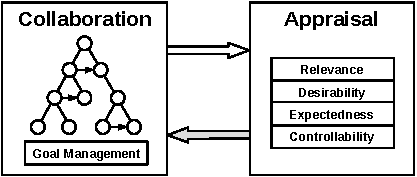
\includegraphics[width=0.8\textwidth]{figure/goal_management_croped.pdf}
  \caption{Using Appraisals' outcome to influence Collaboration structure
  (mechanisms in our framework).}
  \label{fig:appraisal-on-collaboration}
\end{figure}

Here, we describe the goal management process in our framework using an
astronaut-robot collaboration example. We introduce the goal management process
based on a cost function including the influence of affective appraisal and
reverse appraisal processes. Goal management is a crucial part of our
investigation of the reciprocal influence of appraisal on a collaboration
structure (see Figure \ref{fig:appraisal-on-collaboration}).

As we mentioned earlier, we use four appraisal variables including: relevance,
desirability, expectedness and controllability. The outcome of each appraisal
process is a specific value for the corresponding appraisal variable. The vector
containing these appraisal variables can be mapped to a particular emotion
instance at each point in time when requied. Moreover, the functions of emotions
in a social setting, i.e., goal management, and the meaning of the
collaborator's perceived emotion in collaboration context are also important.

A collaboration structure provides a hierarchy and constraints of the shared
goals in the form of a shared plan (Figure \ref{fig:taskModel}) which contains
both the robot and the human collaborator's goals. The robot pursues the goals
for which the robot is responsible in the shared plan. However, there can be
several live goals available for the robot to pursue at each point in time
during collaboration. A goal is live if all of its predecessors are achieved and
all of its preconditions are satisfied. Therefore, a collaborative robot
requires a mechanism to choose between a set of live goals. We believe appraisal
processes are crucial to choose between the available live goals, since the
appraisals are the immediate outcome of the robot's assessment of the
collaboration environment.

\begin{figure}[tbh]
  \centering
  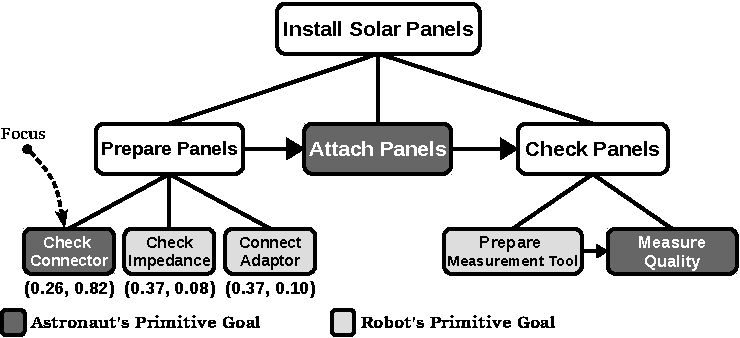
\includegraphics[width=1\textwidth]{figure/goal_management_collaboration_structure-croped.pdf}
  \caption{Cost values indicated by tuples with (second number) and without
  (first number) the influence of emotions.}
  \label{fig:task-model-astronaut}
\end{figure}

For instance, Figure \ref{fig:task-model-astronaut} shows a non-primitive
``Prepare Panels'' goal decomposed into three primitive goals. Therefore, if
``Prepare Panels'' is live, its primitive goals can be pursued by the
responsible agent. In our example, the astronaut is responsible for the ``Check
Connector'' goal; the robot is responsible for the remaining two primitive
goals. According to the collaboration mechanism in our overall framework,
``Check Connector'' is in focus, with the astronaut pursuing this goal.
Suddenly, however the astronaut tells the robot that she can not find the
connector and she is \textit{worried} about failure of this goal. The robot's
response to this situation will be explored below as we discuss details of our
cost function.

Equation \ref{eqn:cost} shows the function to calculate the cost of each
live goal. The base in the equation calculates the cost of pursuing any given
goal. The three functions used to calculate the cost are:
\textit{proximity} $P(g)$, \textit{difficulty} $D(g)$, and \textit{specificity}
$S(g)$ (see equations \ref{eqn:proximity} to \ref{eqn:specificity}).

\begin{equation}
{\fontsize{6}{9}\selectfont Cost(g) =
\big(\omega_0.P(g)+\omega_1.D(g)+\omega_2.\frac{1}{S(g)+1}\big)}^{\Gamma}
\label{eqn:cost}
\end{equation}

\noindent For simplicity, we assume equal values for the weights: $\omega_i$=1.

\begin{equation}
\Gamma=-C[(R_r+1)D_r + \alpha(R_h+1)D_h]
\label{eqn:power}
\end{equation}

The exponent part of our cost function (Equation \ref{eqn:power}) captures a)
the influence of the human's perceived emotional instance, and b) the influence
of self appraisal of the given goal. $R_h\in[0,1]$ and $D_h\in[-1,1]$ are the
relevance and desirability values respectively, which are based on the
\textit{reverse} appraisal of the human's perceived emotion. For instance, if
the astronaut is \textit{worried}, $D_h$ is negative, e.g., -0.8 (depending on
how undesirable the event is according to reverse appraisal), and $R_h$ will be
1 for the active goal and its value descends to 0 for other live goals depending
on their distance to the active goal in the shared plan (e.g., 0.1).

$R_r\in[0,1]$ and $D_r\in[-1,1]$ are relevance and desirability values, provided
by the \textit{self} appraisal functions for all of the live goals. For
instance, for the active goal for which the astronaut was \textit{worried},
$D_r$ can be positive, e.g., 0.8 (depending on the self's desirability appraisal
function); $R_r$ can be 1, since the active goal is relevant for the robot.
These values will change for the other live goals depending on how
relevant they are with respect to the collaboration status (e.g., 0.9 and 0.8).
Finally, $C\in[1,\infty)$ is a constant (e.g., 2) used to control the influence
of affect on cost value. It is negative since undesirability (negative values)
should increase the cost. $\alpha\in[1,\infty)$ is another constant (e.g., 3)
used to control the importance of reverse appraisal relative to self appraisal.

The \textit{proximity} of a goal indicates how far the goal is from the current
active goal in the shared plan. It is calculated by the distance function
(Equation \ref{eqn:proximity}) which returns the number of edges between the
current active goal $g_{_{act}}$, and the given goal $g$ in the shared plan. In
our example, $P(g)$ is 2 for both ``Check Impedance'' and ``Connect Adaptor''
goals.

\begin{equation}
P(g) = max\big\{1, distance(g_{_{act}},g)\big\}
\label{eqn:proximity}
\end{equation}

The \textit{difficulty} of a goal is a function of three parameters (Equation
\ref{eqn:difficulty}) which consider the difficulty based on a) topology of the
shared plan tree (domain independent), and b) the amount of effort required to
pursue a given goal (domain dependent). The $\sum pred_e(g)$ is the sum of
efforts that all the \textit{predecessors} of a given goal $g$ require. The
$\sum desc_e(g)$ is the sum of efforts that all the \textit{descendants} of a
given goal $g$ require. The effort values represent the amount of effort for the
goals with respect to the domain. In our example, we assume the values of all
the goal efforts are 1 for simplicity. The $H(g)$ is the height of the given
goal $g$. The heights of all primitives under ``Prepare Panel'' goal are 0 in
our example.

\begin{equation}
D(g) = \Big(H(g)+1\Big)\times\left[\sum\limits_{m=0}^{M} pred_e(g) +
\sum\limits_{n=0}^{N} desc_e(g)\right]
\label{eqn:difficulty}
\end{equation}

The \textit{specificity} of a goal is the function of \textit{depth} (distance
from the root) and \textit{degree} (number of children in the graph) of a given
goal $g$. The first non-primitive goal (root) is the least specific goal, and
the primitives (leaves) are the most specific goals. As calculated based on
Figure \ref{fig:task-model-astronaut}, the values of $S(g)$ for the three
primitives under the ``Prepare Panels'' are 2.

\begin{equation}
S(g) = \frac{depth(g)}{degree(g)+1}
\label{eqn:specificity}
\end{equation}

The tuples below the goals in Fig. \ref{fig:task-model-astronaut} indicate the
cost value of each goal. The first number in each tuple is the normalized cost
value without the influence of the affective part of the cost function, i.e.,
the exponent is equal to 1 in Equation \ref{eqn:cost}. The second number of each
tuple indicates the normalized value of the cost including the influence of
affective appraisal and the astronaut's perceived emotion.

Based on our cost function, the cost of completing the primitive goal ``Check
Connector'' is 0.82 (see Figure \ref{fig:task-model-astronaut}). As shown, when
affect is not considered the cost is 0.26; the negative emotion of the astronaut
(worry) significantly increases the cost of the current goal, and also impacts
the other two primitive live goals under the same parent. Therefore, instead of
insisting on pursuing the same blocked goal which has caused the astronaut's
negative emotion, the robot can mitigate the astronaut's emotions by adapting to
her worry. The robot shifts the focus of attention to ``Check Impedance'' to
maintain progress and prevent failure of the collaboration.

We use our proposed cost function in our goal management algorithm to integrate
affective appraisal into the collaboration mechanism in our framework. A similar
situation is used in our conducted user study (see Chapter \ref{ch:awareness})
to evaluate the human's perception of the robot's behavior as a result of the
goal management process.

\section{Coping Mechanism and Strategies}
We have implemented Coping mechanism to determine how the agent would respond to
the events using our framework. Our Coping mechanism includes a set of coping
strategies that can be triggered based on different conditions (see Figure
\ref{fig:coping_strategies}). All of these coping strategies are known in the
literature. Some of our coping strategies, i.e., \textit{planning},
\textit{active coping} and \textit{seeking social support for instrumental
reasons}, are categorized as problem-focused and some others, i.e.,
\textit{acceptance}, \textit{mental disengagement}, \textit{shifting
responsibility}, and \textit{wishful thinking}, are categorized as
emotion-focused startegies as described in \cite{gratch:domain-independent}.

In our Coping mechanism, there are three components involved as the activation
criteria for each coping strategy. The first criterion is the conjunction of
emotion valances of the self and the other collaborator (see Emotion Valance
column in Figure \ref{fig:coping_strategies}). For instance, if the valance of
the human collaborator's emotion is \textit{negative} \textbf{and} the valance
of the agent's emotion is also \textit{negative}, the active coping, the
acceptance, and the mental disengagement coping strategies are the coping
strategy candidates that have potential to become activated if the other
activation criteria also exist for any of them. For example, if the human
collaborator is frustrated and the agent's elicited emotion is guilt, the three
above mentioned coping strategies become potential candidate to be selected as
the agent's active coping strategy. The second criterion is the need for the
agent to cope with an event. The values of our three different motives (i.e.,
\textit{satisfaction}, \textit{achievement}, and \textit{external}) are involved
in the decision of whether there is a need for a particular coping strategy to
become activated. We use conjunction of satisfaction motive's value with the
disjunction of achievement and external motives. For instance, if we have highly
negative values for all three motives for the potential candidates of coping
strategies based on the example we mentioned above, the acceptance coping
strategy will be selected as the strategy with the highest need for the agent.
For example, this kind of condition can occur when the agent fails doing its own
task and pursuing the current goal (negative satisfaction motive), and can not
find another goal to overcome the impasse (negative achievement motive). The
details about how the motive values are computed is presented in Section
\ref{sec:motivation_mechanism}. Finally, the ability to cope with an event as
the third criterion impacts the decision of whether the selected coping startegy
can be activated. The controllability of an event represents whether the agent
is able to control the situation occurring with the given event. In our
example, if the agent finds the event uncontrollable, the acceptance coping
strategy becomes activated (see Figure \ref{fig:coping_strategies}).

\begin{sidewaysfigure}
  \centering
  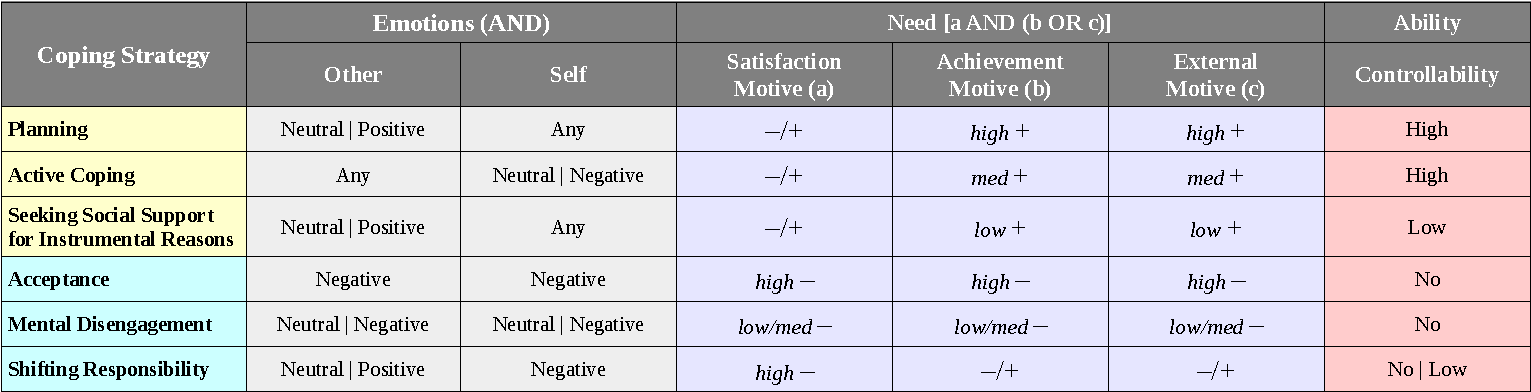
\includegraphics[width=1\textwidth]{figure/coping_algorithms_short_croped.pdf}
  \caption{Conditions for selecting coping strategies}
  \label{fig:coping_strategies}
\end{sidewaysfigure}

\section{Other Mechanisms in our Architecture}

\subsection{Motivation}
\label{sec:motivation_mechanism}

\subsection{Theory of Mind}
The Theory of Mind mechanism uses the same collaboration structure and functions
as well as appraisal processes to form anticipated beliefs about human's mental
and emotional states. The agent uses the collaboration structure during the
human's turn to compute appraisal values with respect to the human's current
goal in the shared goal structure. The outcome of this appraisal forms beliefs
about anticipated mental and emotional state of the human collaborator.

\subsection{Perception and Action}

\section{Emotion Instances}
We have also implemented 10 different emotion instances that can be elicited by
the agent or anticipated from the human during collaboration in our framework
(see Figure \ref{fig:emotion_elicitation}). These emotion instances have
meanings in social context and more specifically in collaboration. There are two
components involved in selecting a particular emotion: appraisal variables and
collaboration context.

We use the outcome of the four appraisal processes discussed in section
\ref{sec:appraisal} to determine the potential emotion instance to be elicited
(if the agent wants to express an emotion), or to anticipate a potential emotion
from human collaborator (if the human response is anticipated). The outcome of
appraisal processes can be one of the values presented in Figure
\ref{fig:appraisal_values} with respect to the corresponding process.

\begin{figure}[tbh]
  \centering
  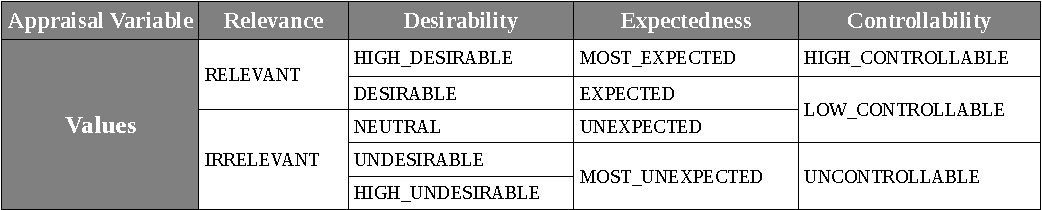
\includegraphics[width=1\textwidth]{figure/apraisal_values_croped.pdf}
  \caption{Appraisal values.}
  \label{fig:appraisal_values}
\end{figure}

We also use the collaboration context as our second determinant of selecting a
particular emotion. We define the collaboration context based on: \textit{goal
achievement}, \textit{goal failure}, \textit{proposal of a goal},
\textit{acceptance of the proposed goal}, and \textit{rejection of the proposed
goal}. All of these situations can occur by either of the collaborators, i.e.,
agent or human (see Figure \ref{fig:emotion_elicitation}). There is only one
exception and it is when the desirability value is neutral the associated
emotion to the event is always neutral without considering the collaboration
context and the values of other appraisal variables.

As an example, if the agent finds an event \textit{uncontrollable},
\textit{unexpected}, \textit{undesirable} and \textit{relevant} as the result of
human's proposal of a new goal to the agent (in agent's turn), the elicited
emotion instance will be \textit{worry} which can be expressed by the agent to
indicate the agent's concern. Similarly, the agent will anticipate
\textit{worry} for the human if the same appraisal values are computed while for
instance the agent rejects human's proposal of the new goal (in human's turn).


\begin{sidewaysfigure}
  \centering
  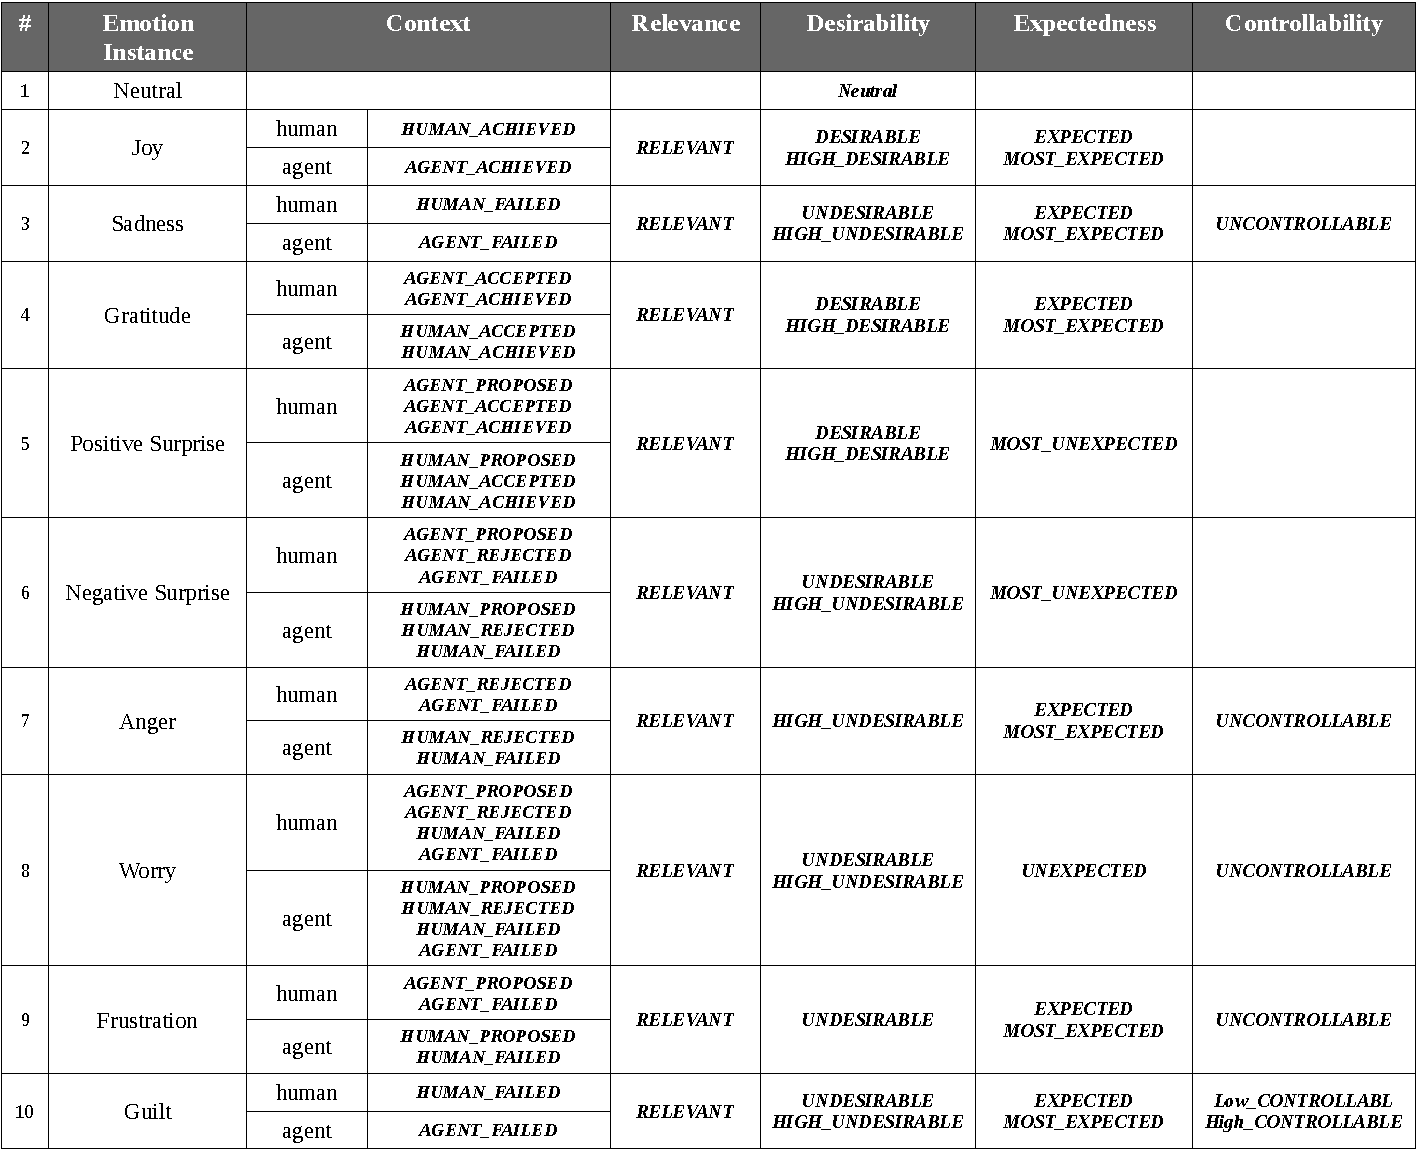
\includegraphics[width=1\textwidth]{figure/emotion_elicitation_croped.pdf}
  \caption{Conditions for selecting emotion instances}
  \label{fig:emotion_elicitation}
\end{sidewaysfigure}

\section{Experimental Scenario}
We developed an experimental scenario to in which participants were asked to
carry out a sequence of hypothetical collaborative tasks between themselves and
an imaginary friend, Mary, in order to accomplish their shared goal. To minimize
the background knowledge necessary for our test subjects, we used a simple
domestic example of preparing a peanut butter and jelly sandwich, and a hard
boiled egg sandwich for a hiking trip. The tasks did not require the
participants to solve problems; rather, the tasks were part of simple daily
activities that should be familiar to all participants. 
% 
% \subsection{Tasks}
% Participants were asked to carry out a sequence of hypothetical collaborative
% tasks between them and an imaginary friend, Mary, in order to accomplish their
% goal of preparing two sandwiches. All the tasks were simple and did not require
% the participants to solve a particular problem rather accomplish something as
% they do in their day to day life.
% 
% \section{Evaluation}

\subsection{Hypothesis}
We conducted this user study to test our hypothesis that humans and our
algorithms will provide similar answers to questions related to different
factors used to compute four appraisal variables: relevance, desirability,
expectedness, and controllability.

\begin{figure*}[tbh]
  \centering
  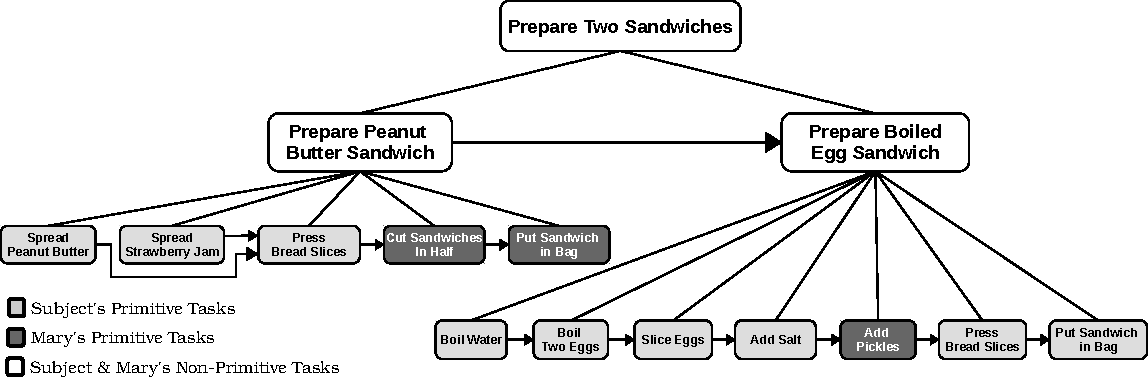
\includegraphics[width=1\textwidth]{figure/taskModel-croped.pdf}
  \caption{Collaboration Task Model for the Evaluation.}
  \label{fig:taskModel}
\end{figure*}

\subsection{Procedure}
 We conducted a between-subject user study using an online crowdsourcing website
 -- CrowdFlower\footnote{http://www.crowdflower.com}. We had a questionnaire for
 each appraisal variable. There were 12 questions (including 2 test questions)
 in the controllability and expectedness questionnaires, 14 questions (including
 2 test questions) in the desirability questionnaire, and 22 questions
 (including 3 test questions) in the relevance questionnaire.
 
We provided textual and graphical instructions for all questionnaires; Figure
\ref{fig:taskModel} shows the corresponding task model. The instructions,
provided in Figure XXX, presented a sequence of hypothetical collaborative tasks
to be carried out by the test subject and an imaginary friend, Mary, in order to
accomplish their goal of preparing two sandwiches. We also provided a simple
definition and an example of each appraisal variable. The collaboration
structure and the instructions were the same for all questionnaires. The
questions introduced specific situations related to the shared plan, which
included blocked tasks and failure or achievement of a shared goal. Each
question provided three answers which were counterbalanced in the questionnaire.
We provided an option like C in all questions (see Figure \ref{fig:qs1}),
because we did not want to force participants to choose between two options when
they did not have a good reason. There were two questions designed based on each
factor that we use in our algorithms (see Section \ref{sec:appraisal}). The
questions were randomly placed in the questionnaire. Figure \ref{fig:qs1} shows
an example question from the relevance questionnaire which was designed to test
whether participants perceive saliency as a factor in relevance. The input for
our algorithms was the task model depicted in Figure \ref{fig:taskModel}.

\subsection{Participants}
Each participant group originally had 40 participants. We limited the
participant pools to those with the highest confidence level on the
crowdsourcing website in the United States, Britain, and Australia. Test
questions were included to check the sanity of the answers. We eliminated
participants providing wrong answers to our sanity questions, and participants with
answering times less than 2 minutes. The final number of accepted participants
in each group is provided in Table \ref{tbl:statistics}.

\begin{table}[htbp]
\centering
\caption{Number of Participants}
\begin{tabular}{|c|c|c|c|c|} \hline
appraisal variables & \# of participants\\ \hline 
Relevance &  29\\ \hline
Desirability & 35\\ \hline 
Expectedness & 33\\ \hline 
Controllability & 33\\ \hline
\end{tabular}
\label{tbl:statistics}
\end{table}

% \begin{table}[htbp]
% \vspace*{-3mm}
% \centering
% \caption{Number of Participants}
% \begin{tabular}{|c|c|c|c|c|} \hline
% appraisal variables & \# of participants & mean & stdev & \textit{p}-value\\ \hline 
% Relevance &  29 & 0.713 & 0.107 & $<$0.001\\ \hline
% Desirability & 35 & 0.778 & 0.150 & $<$0.001\\ \hline 
% Expectedness & 33 & 0.785 & 0.120 & $<$0.001\\ \hline 
% Controllability & 33 & 0.743 & 0.158 & $<$0.001\\ \hline
% \end{tabular}
% \label{tbl:statistics}
% \vspace*{-3mm}
% \end{table}
% 

\section{Results}
\label{sec:results-crowdsourcing}
Each question in our questionnaires was designed based on different factors that
we use in our algorithms (see Section \ref{sec:appraisal}).  For each of the
four questionnaires we provide an example question, and describe how each
question relates to a specific factor within the corresponding algorithm. The
input for our algorithms was the task model depicted in Figure
\ref{fig:taskModel}. The complete list of questions is provided in the Appendix.
Additionally, we provide the p-value for each question, using a binomial
distribution, with a probability of success of 0.33, which is the probability of
selecting the right answer if the participant is simply guessing.

\subsection{Expectedness}
\label{sec:expectedness-crowdsourcing}
Figure \ref{fig:qs1} shows an example question from the expectedness
questionnaire. In this example, with respect to Algorithm
\ref{alg:expectedness} (line 6), option A is more expected because the task
related to this option provides the next available task in the focus stack (see
the task model in Figure \ref{fig:taskModel}). Although the task in option B is
part of the existing task model, it is considered as unexpected by our
algorithm, since it is not live in the plan. We provided option C to determine
whether the participants will similarly differentiate between these two
options. This question was presented to the participants to determine whether
their decision for the expectedness of this event is similar to the output of
the expectedness algorithm. For this question, the human decision was 97\%
similar to the algorithm's output. 

\begin{figure}[tbh]
  \centering
  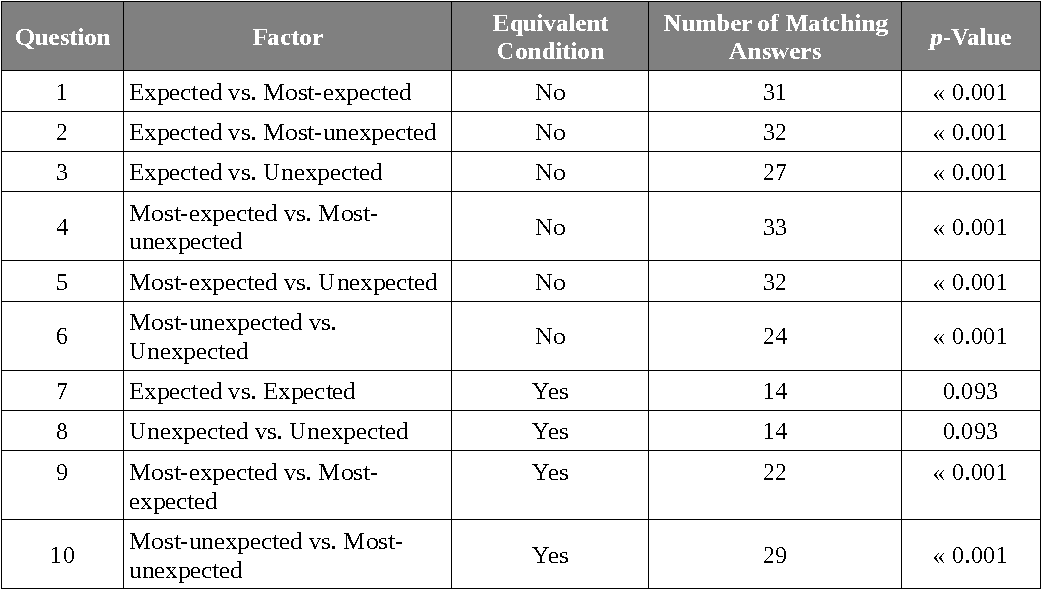
\includegraphics[width=1\textwidth]{figure/expectedness_result_croped.pdf}
  \caption{Expectedness results.}
  \label{fig:expectedness_result}
\end{figure}

Results for the expectedness questionnaire are presented in Table XXX (Refer to
Expectedness summary table). As shown in this table, there is strong evidence
that the results are not random; in fact, for questions 1-6 and 9-10, human
participants showed between 67 and 100 \% agreement with our algorithms, with
p-values of <<0.001 when compared with a random population. Questions 7 and 8
were the only two questions that did not show a statistically significant
p-value. It should be noted that these questions are comparing equally expected
or equally unexpected situations, none of which our algorithms would consider
most-expected or most-unexpected. 


\begin{figure}[tbh]
  \centering
  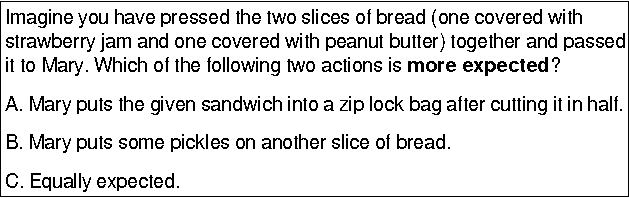
\includegraphics[width=0.85\textwidth]{figure/question-sample-croped.pdf}
  \caption{{\fontsize{9}{9}\selectfont Example Expectedness Question.}}
  \label{fig:qs1}
\end{figure}

\subsection{Controllability}
\label{sec:controllability-crowdsourcing}
Figure \ref{fig:qs2} shows an example question from the controllability
questionnaire. The algorithm's output is option B, and is determined by
Algorithm \ref{alg:controllability} (line 3), similarly to the expectedness
example above. In this example, option B is more controllable than option A,
because the self over total ratio of the responsibility of the predecessors of
the given task (see \textit{Autonomy} in Section \ref{sec:controllability}) is
higher than the ratio in option A; i.e., self is responsible to spread peanut
butter on one slice of bread and strawberry jam on another slice of bread. In
this question, the humans decision was 90\% in agreement with the algorithm's
output.

\begin{figure}[tbh]
  \centering
  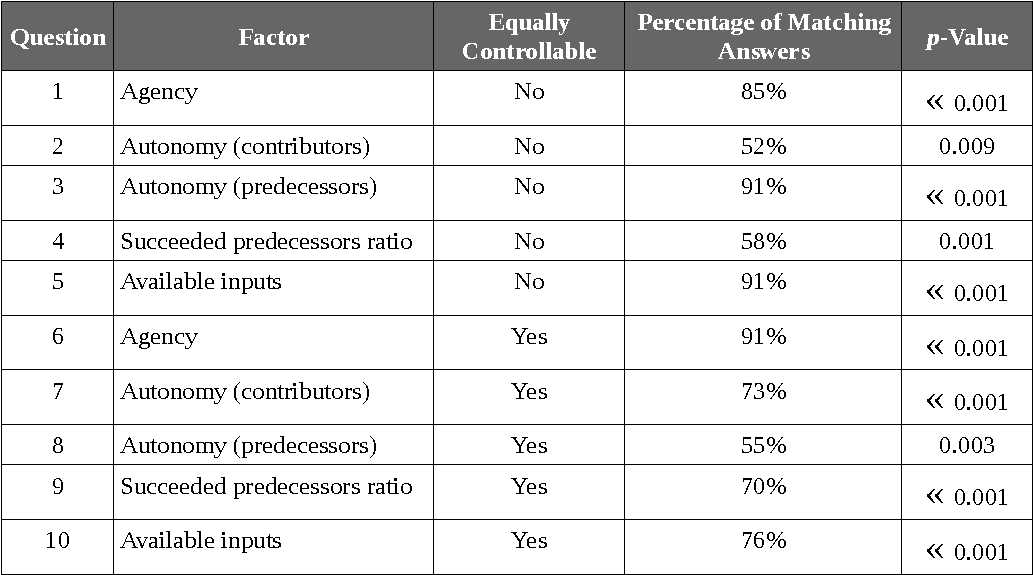
\includegraphics[width=1\textwidth]{figure/controllability_result_croped.pdf}
  \caption{Controllability results.}
  \label{fig:controllability_result}
\end{figure}

Results for the controllability questionnaire are presented in Table XXX
(insert controllability summary table). As shown in the table, the p-value is
<0.01 for each of the ten questions. The two questions with the lowest human
agreement with the algorithms both relate to autonomy of the participants with
52\% and 55\%. 

\begin{figure}[tbh]
  \centering
  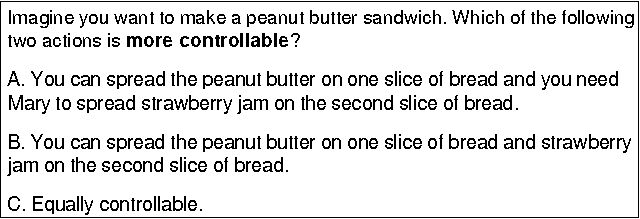
\includegraphics[width=0.85\textwidth]{figure/question-sample2-croped.pdf}
  \caption{{\fontsize{9}{9}\selectfont Example Controllability Question.}}
  \label{fig:qs2}
\end{figure}

\subsection{Desirability}
\label{sec:desirability-crowdsourcing}
Figure \ref{fig:qs3} shows an example question from the desirability
questionnaire. The output based on the Algorithm \ref{alg:desirability}
(line 14) is option C, since in both option A and option B, the focus goal
has been achieved successfully. Therefore, in this example, both options A and B
are desirable. The humans' decision was 77\% in agreement with the algorithm's
output in this question.

\begin{figure}[tbh]
  \centering
  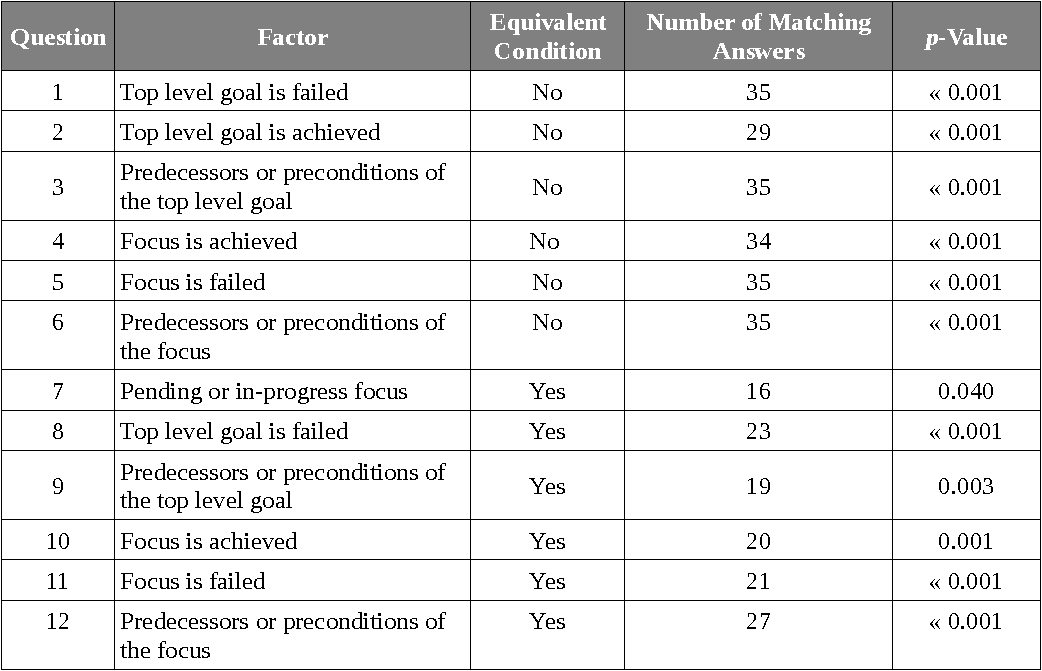
\includegraphics[width=1\textwidth]{figure/desirability_result_croped.pdf}
  \caption{Desirability results.}
  \label{fig:desirability_result}
\end{figure}

The results of the desirability questionnaire are presented in Table XXX
(insert desirability summary table). As shown in the results table, the p-value
is less than 0.05 for all of the desirability questions. However, an interesting
trend is that human participants had a level of agreement of 83\%-100\% when the
algorithm's output selected one alternate as more desirable than another
alternate. When the algorithm's output chose option C (i.e. rating two
situations as equally desirable), the human participants only showed 46\%-77\%
agreement. This may indicated that a higher level of granularity is required in
the algorithm when evaluating options with similar levels of desirability. 

\begin{figure}[tbh]
  \centering
  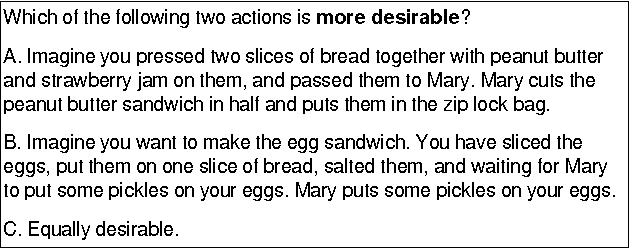
\includegraphics[width=0.85\textwidth]{figure/question-sample3-croped.pdf}
  \caption{{\fontsize{9}{9}\selectfont Example Desirability Question.}}
  \label{fig:qs3}
\end{figure}

\subsection{Relevance}
\label{sec:relevance-crowdsourcing}
In the example shown in Figure \ref{fig:qs4}, with respect to Algorithm
\ref{alg:relevance}, option A is relevant because of Mary's perceived negative
emotion (see Equation \ref{eqn:utility}). Although option B is relevant (since
it achieves the next goal in the shared plan), 83\% of participants consider it as
less relevant than option A; we believe this is due to the effect of Mary's
perceived negative emotion which also generates a higher utility value in our
relevance algorithm. Another question also tested belief saliency. However, the
options provided only related to the shared plan (i.e., no human emotions in the
options). In this case 87\% of participants chose the option that accomplished the
next goal in the shared plan. Interestingly, when confronted with a negative
emotion from their collaborator, human participants deviated from the shared plan
and found their collaborator's emotion more relevant than the original plan. It
is noteworthy that in both the absence and the presence of emotions the
participants chose the more salient option with respect to our definition of
saliency, which was not referenced or provided in the questionnaire.

\begin{figure}[tbh]
  \centering
  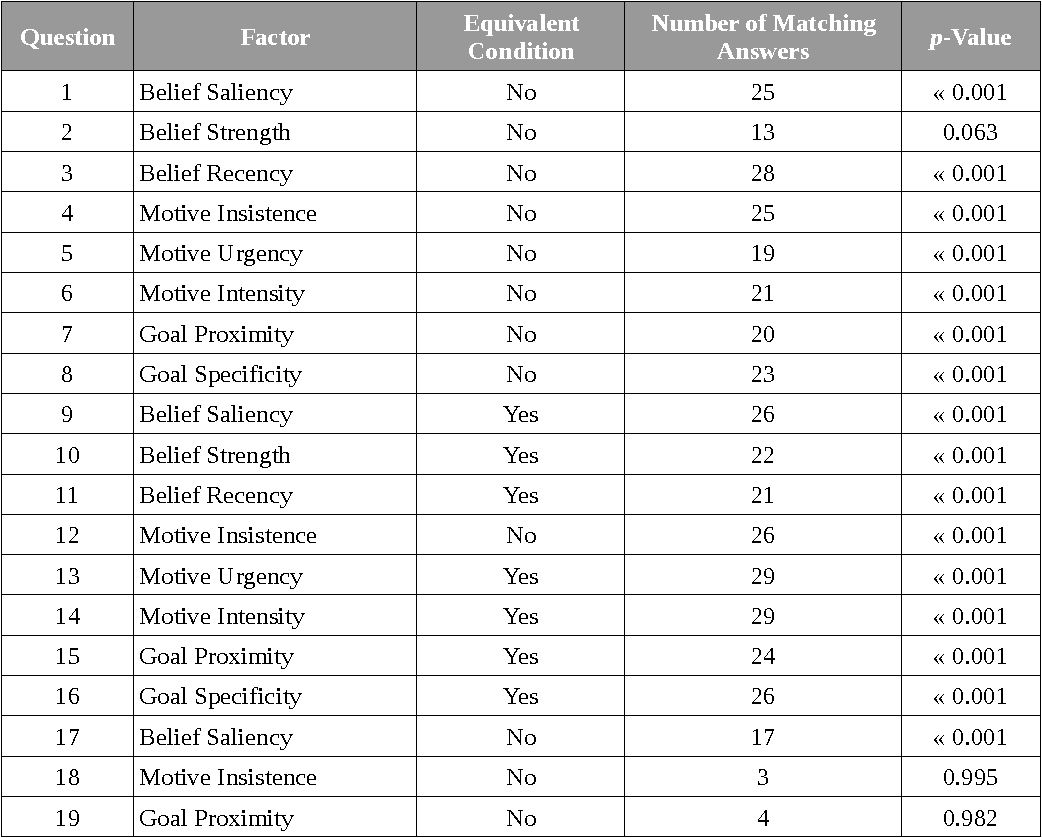
\includegraphics[width=1\textwidth]{figure/relevance_result_croped.pdf}
  \caption{Relevance results.}
  \label{fig:relevance_result}
\end{figure}

The complete summary of results for the relevance questionnaire is provided in
Table XXX (Insert summary table for relevance). As shown in the table, all
questions show 59\%-100\% agreement with our algorithms and statistically
significant p-values except for questions 2, 18 and 19. Question 2 addresses
belief strength. Questions 18 and 19 address motive insistence and goal
proximity, respectively; both of these questions present situations in which
participants must choose whether an intense emotional circumstance, or adherence
to the collaboration plan is more relevant (refer to the questionnaire
provided in the Appendix). Our algorithms choose that the strong emotional
circumstance will be more relevant; however, human participants generally
selected adherence to the collaboration plan to be more relevant. 

\begin{figure}[tbh]
  \centering
  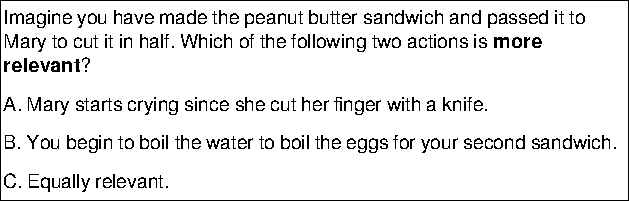
\includegraphics[width=0.85\textwidth]{figure/question-sample4-croped.pdf}
  \caption{{\fontsize{9}{9}\selectfont Example Relevance Question.}}
  \label{fig:qs4}
\end{figure}

\section{Discussion}
\label{sec:discussion-crowdsourcing}
As shown in the results tables in sections \ref{sec:expectedness-crowdsourcing}
through \ref{sec:relevance-crowdsourcing}, the human participants agreed 100\%
on some questions, while on some other questions there was a much lower level of
agreement. Our results indicate that people largely performed as our hypothesis
predicted. The \textit{p}-values obtained based on a binomial distribution show
the probability of human participants' answers being generated from a random
set. The very small \textit{p}-values indicate that the data set is not random;
in fact, the high percentage of similarity confirms our hypothesis and shows
that the algorithms can help us to model appraisal in a collaboration. The very
low level of agreement on a handful of questions may indicate algorithm
components that require further refinement before implementation. 

\section{Conclusions}
\label{sec:conclusions-crowdsourcing}

\chapter{Improving Human-Robot Collaboration Using Emotional-Awareness}
\label{ch:awareness}

\section{Introduction}

As mentioned earlier, collaborative robots need to take into account humans'
internal states while making decisions during collaboration. Humans express
emotions to reveal their internal states in social contexts including
collaboration \cite{breazeal:sociable-interactive-robots}. Due to the existence
of such expressions robots' emotional-awareness can improve the quality of
collaboration in terms of humans' perception of performance and preferences.
Hence, collaborative robots need to include affect-driven mechanisms in their
decision-making processes to be able to interpret and generate appropriate
responses and behaviors. Our aim in this setup was to study the importance of
emotional awareness and the underlying affect-driven processes in human-robot
collaboration. We examined how emotional-awareness impacts different aspects of
humans' preferences by comparing the results from our participants collaborating
with an emotion-aware and an emotion-ignorant robot.

% \section{Collaborative Behaviors and Emotional-Awareness}
% 
% \subsection{Goal Postponement}
% 
% \subsection{Goal Management}
% 
% \subsection{Task Delegation}
% 
\section{Implementation}
The implementation of this user-study included three separate parts. The first
part incorporated the Affective Motivational Collaboration Framework consisting
of all Mental Processes (see left-side of Figure \ref{fig:framework}) as we
described in Chapter \ref{ch:framework}. The second part was implemented to
receive action commands from the framework and forward them to the robot to
control joints and actuators (see right-side of Figure \ref{fig:framework}).
A wizard was the third part of this setting. The wizard did nothing but inform
the robot/framework whether the current task performed by either the robot or
the participant was achieved successfully. The wizard was completely invisible
to the participants, and the wizard had no impact on the robot's decision other
than providing input regarding tasks' failure or success.

\begin{figure*}[tbh]
  \centering
  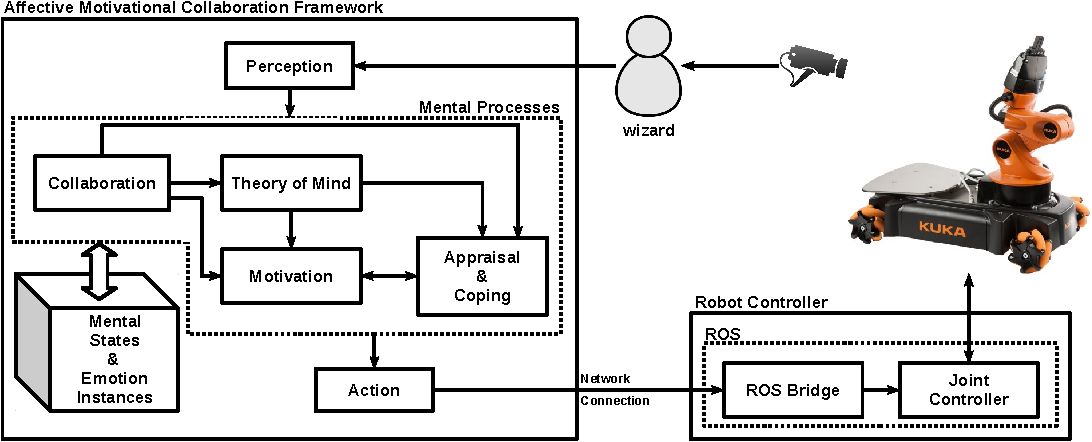
\includegraphics[width=\textwidth]{figure/framework-croped.pdf}
  \caption{\fontsize{10}{10}\selectfont Computational framework based on
  Affective Motivational Collaboration theory (arrows indicate primary
  influences between mechanisms and data flow).}
  \label{fig:framework}
\end{figure*}

\subsection{Framework}
\label{sec:theory}
The framework includes all of the mechanisms depicted as mental processes in
Figure \ref{fig:framework} along with the mental states. The mental
states shown in Figure \ref{fig:framework} comprise the knowledge base required
for all of the mechanisms in the overall model. The details about these mental
processes and mental states are described in Chapters \ref{ch:amct} and
\ref{ch:framework}. In this user-study, the Collaboration mechanism uses a
hierarchy of goals associated with tasks in the hierarchical task network
structure depicted in Figure \ref{fig:collaboration_structure}.

\begin{figure*}[tbh]
  \centering
  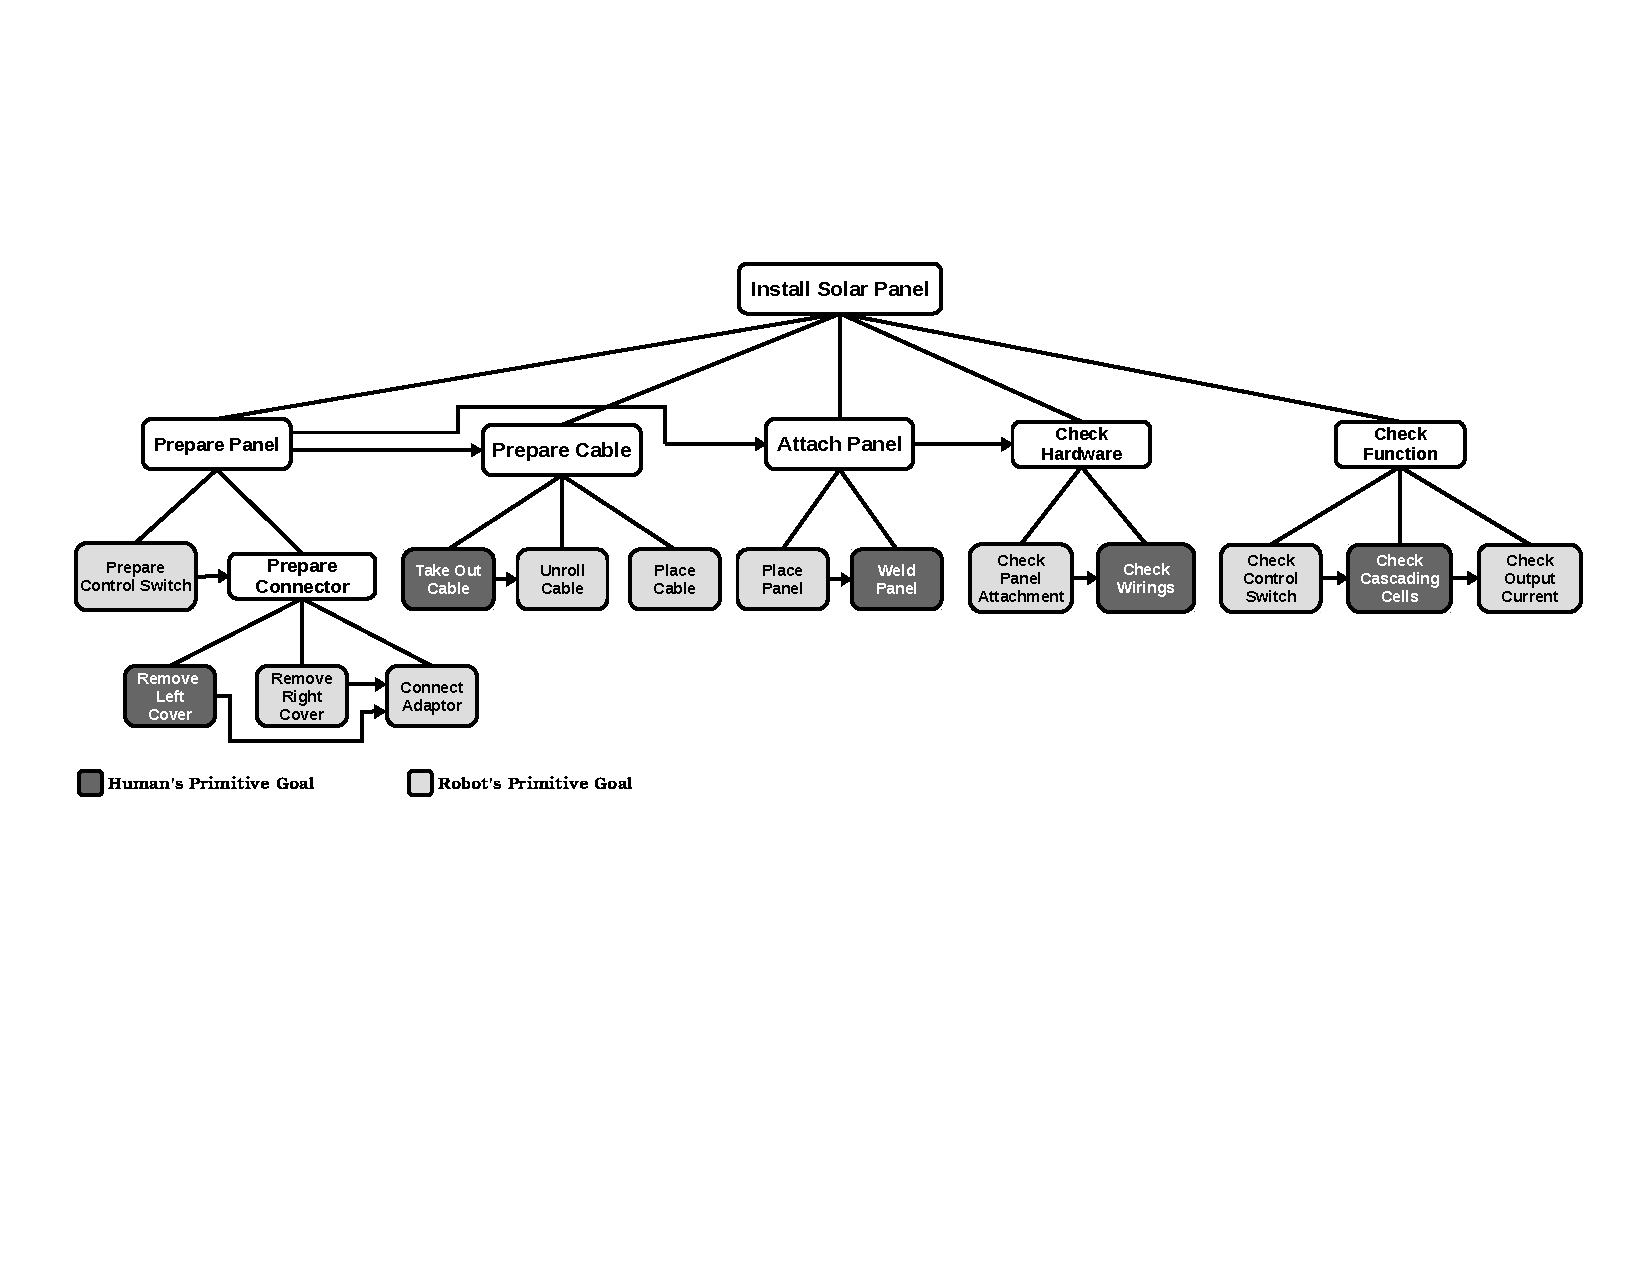
\includegraphics[width=1\textwidth]{figure/collaborationStructure.pdf}
  \caption{{\fontsize{10}{10}\selectfont Collaboration structure used as the
  task model.}}
  \label{fig:collaboration_structure}
\end{figure*}

\subsection{Robot Controller}
The robot controller is comprised of two major components: 1) ROS-bridge and 2)
joint controller (see Figure \ref{fig:framework}).
ROS-bridge\footnote{http://wiki.ros.org/rosbridge\_suite} provides an API to ROS
functionality for non-ROS programs which enables us to send action commands from
our framework (implemented in JAVA) to the robot's joint controller. The joint
controller receives action commands and translates them into actual joint and
actuator commands and sends them to the robot.

\section{Experimental Scenario}

Our scenario was based on a table top turn-taking game that we designed to
simulate the installation of a solar panel. Participants collaborated one-on-one
with our robot to complete all the given tasks required to install the solar
panel. All of the tasks consisted of picking up and placing collaborators'
available pegs on predefined spots on the board (see Figure
\ref{fig:game_board}). Each pick-and-place was associated with the robot's or
the participant's task. The robot and the participants had their own unique
primitive tasks that they had to accomplish in their own turns. The final goal
of installing a solar panel required the robot and the participants to
accomplish their own individual tasks. Failure of any task could create an
impasse during the collaboration.

\begin{figure}[tbh]
  \centering
  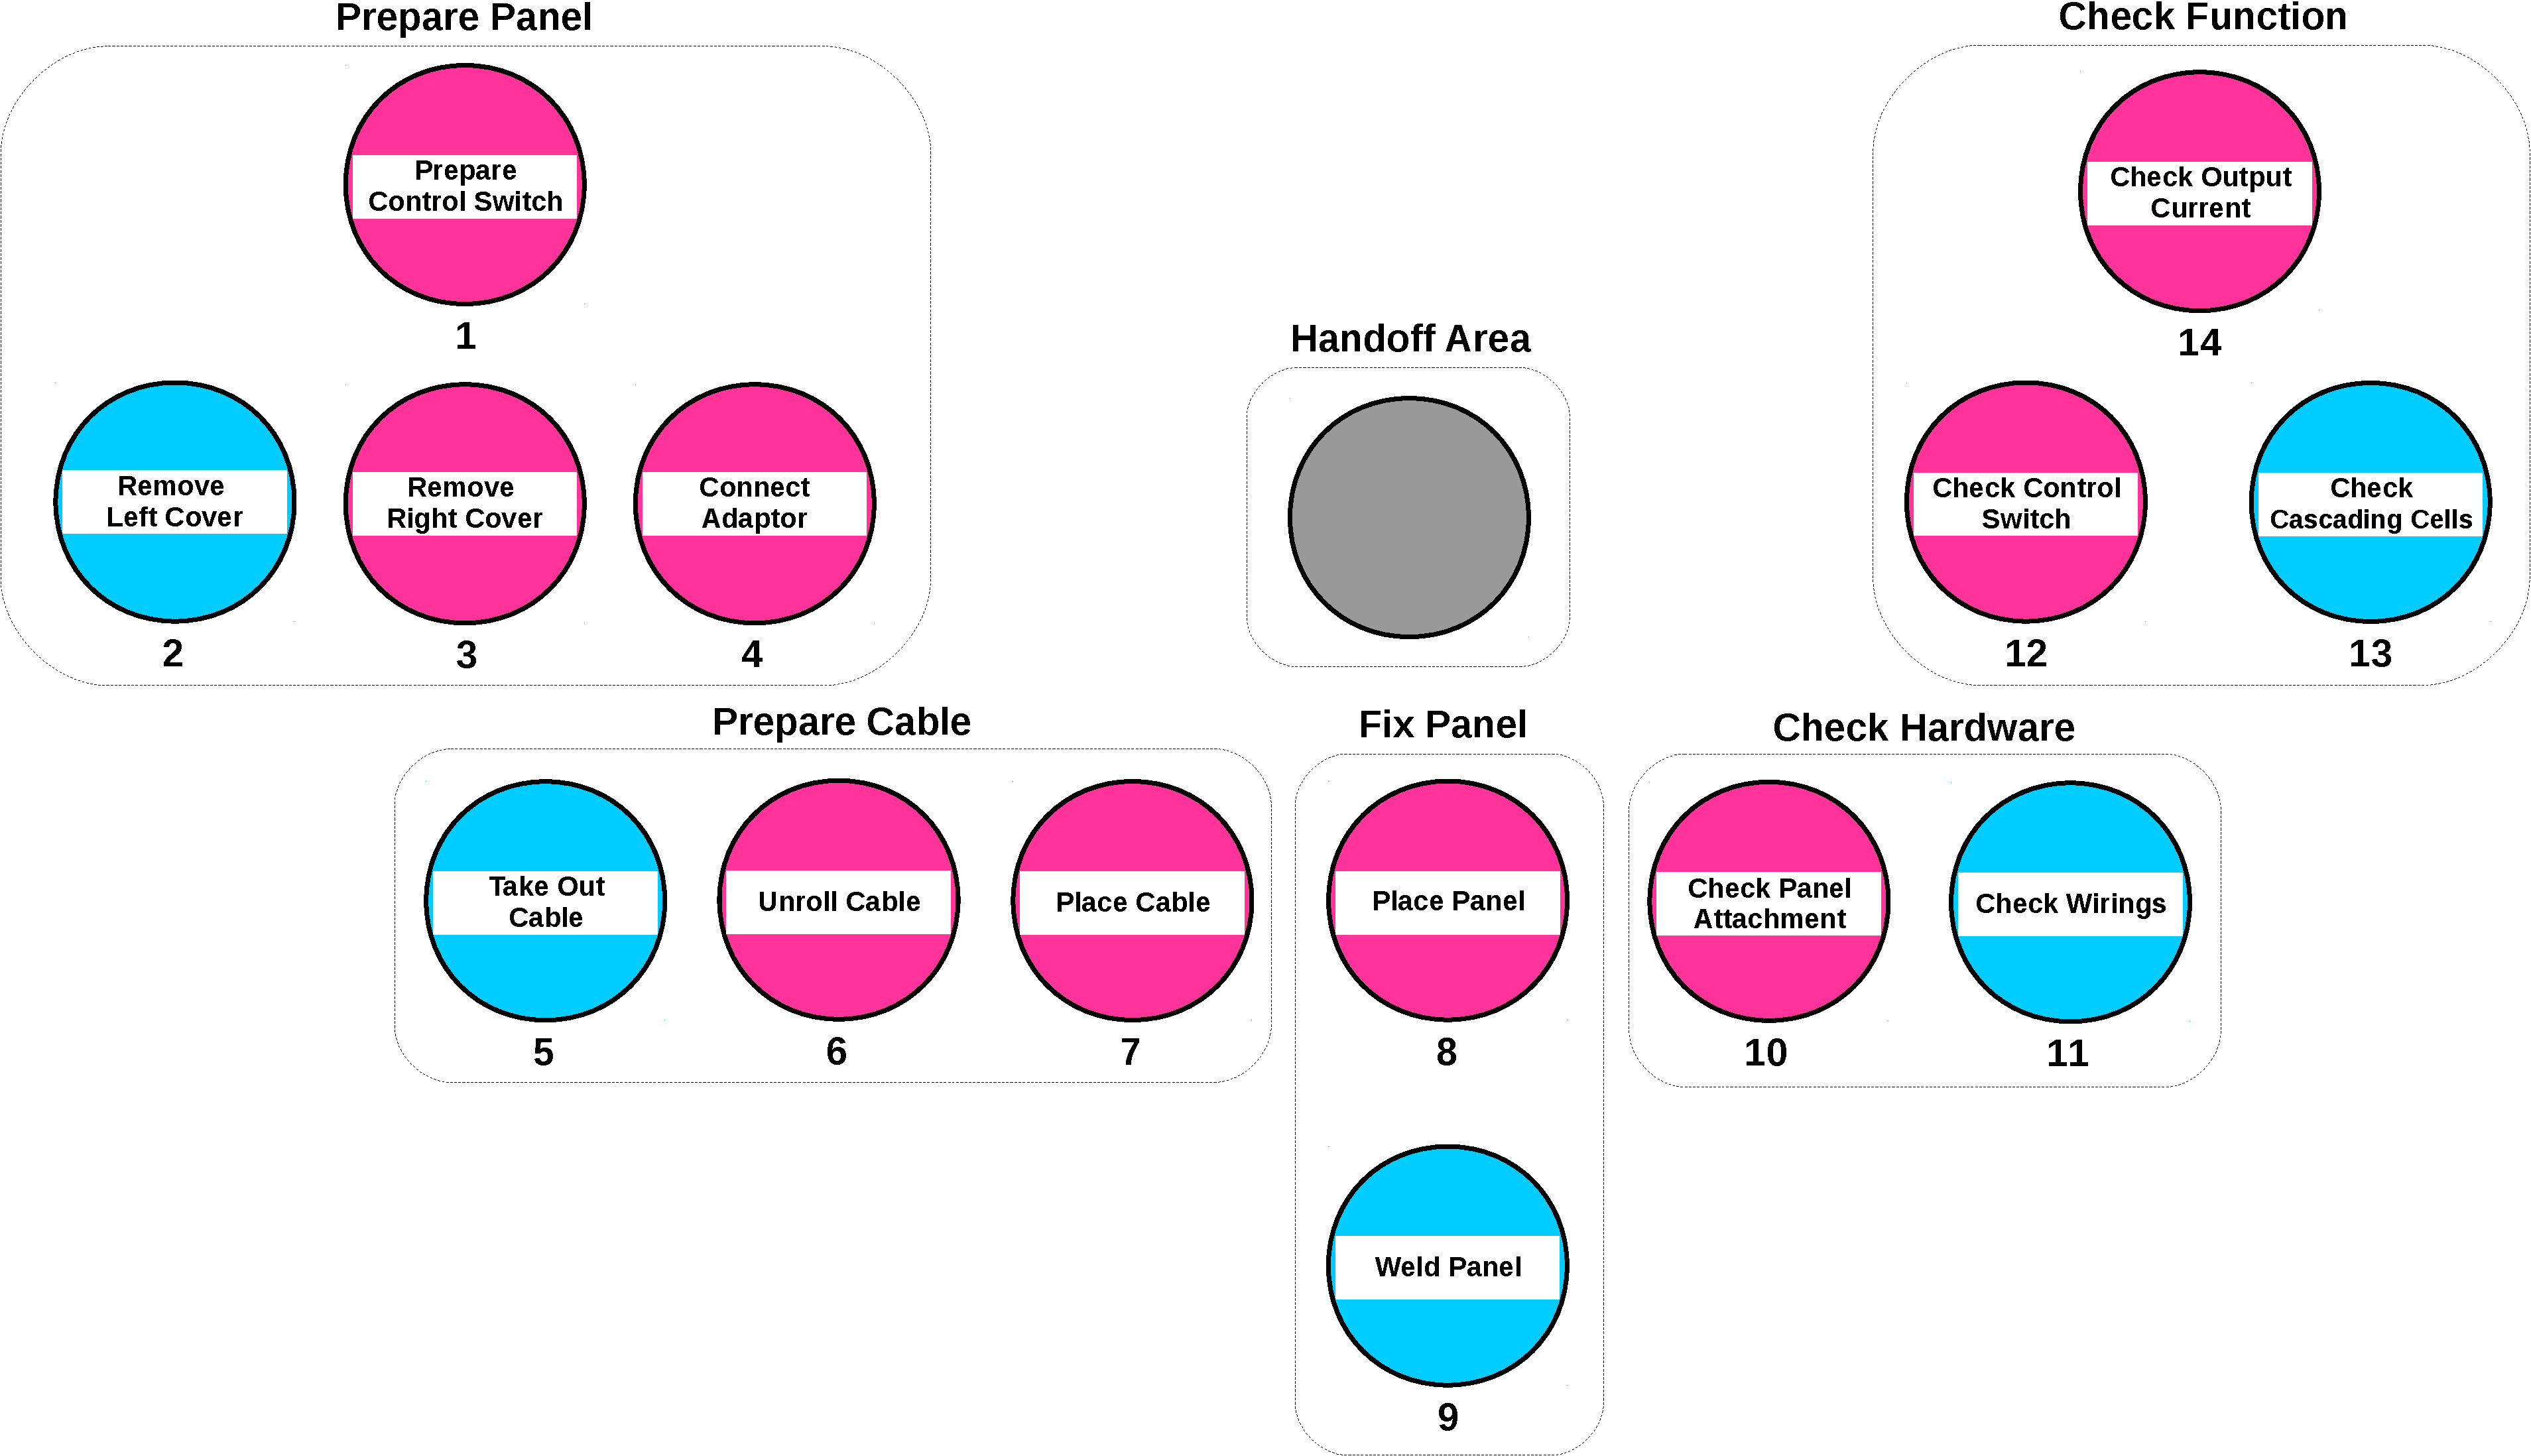
\includegraphics[width=1\textwidth]{figure/gameBoard.pdf}
  \caption{\fontsize{10}{10}\selectfont The layout of the available spots for
  the human and the robot to place their pegs during the collaboration.}
  \label{fig:game_board}
\end{figure}

\subsection{The Robot}

We conducted our experiment based on a KUKA Youbot (see Figure
\ref{fig:environment}). The robot was stationary on top of a desk and was able
to pick up and place available pegs corresponding to the robot's task. The robot
was operated based on Robot Operating System (ROS -- indigo) and was receiving
commands through the ROS-bridge from our Affective Motivational Collaboration
framework (see Figure \ref{fig:framework}). We provided a simple GUI using a
touch-screen monitor (see Figure \ref{fig:gui} and) to a) express the robot's
positive, negative or neutral emotion through an emoticon, b) display the
robot's utterances, c) control turn-taking process of the collaboration, and d)
let the participants express (report) their positive, negative or neutral
emotion for each turn. The robot used MaryTTS an open-source, multilingual
Text-to-Speech Synthesis platform to provide corresponding speech for its
utterances in English.

\begin{figure}
\centering
\begin{subfigure}{.5\textwidth}
  \centering
  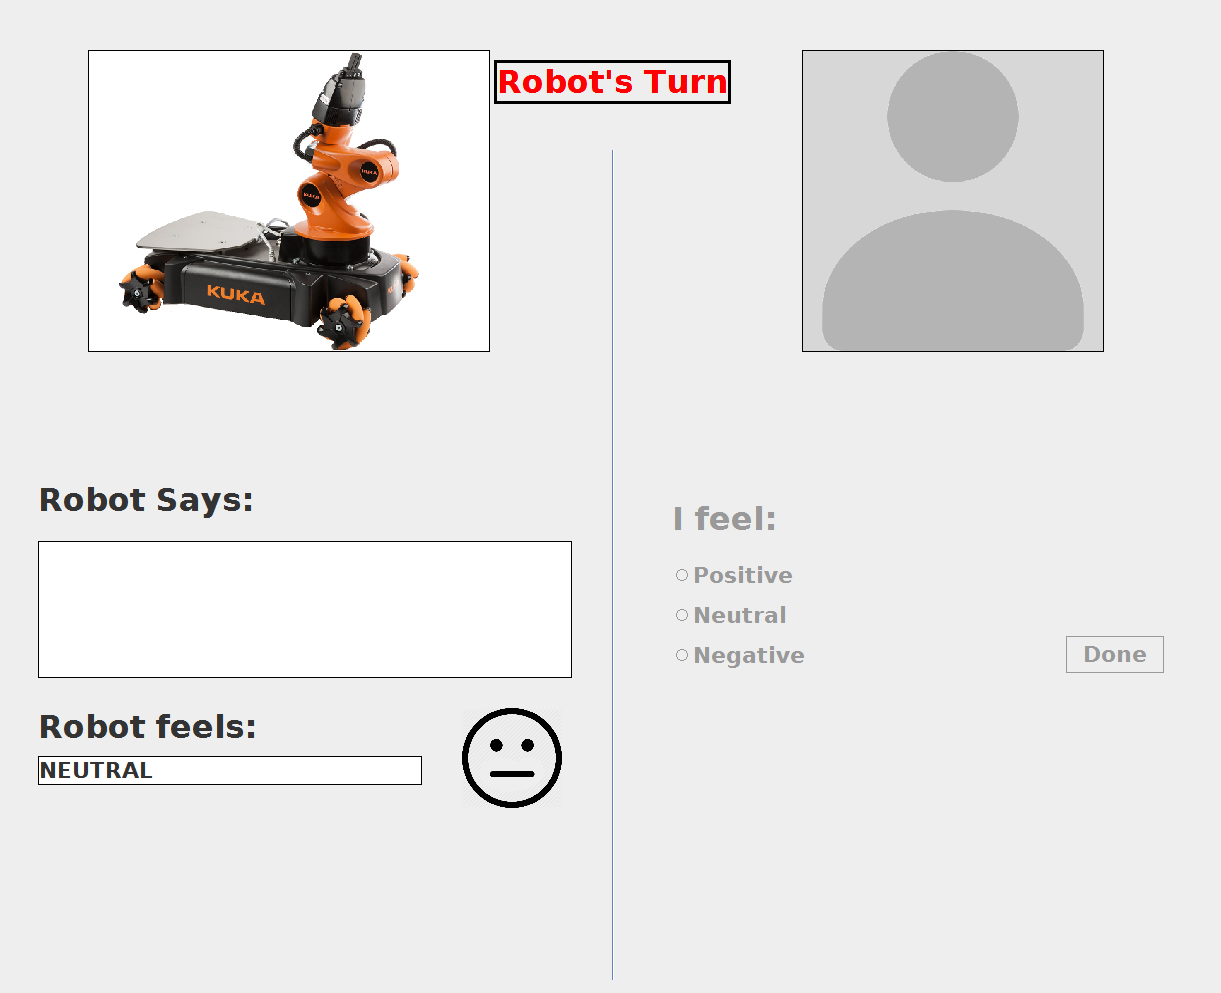
\includegraphics[width=.95\linewidth]{figure/robot-turn-gui.png}
  \label{fig:gui-robot}
\end{subfigure}%
\begin{subfigure}{.5\textwidth}
  \centering
  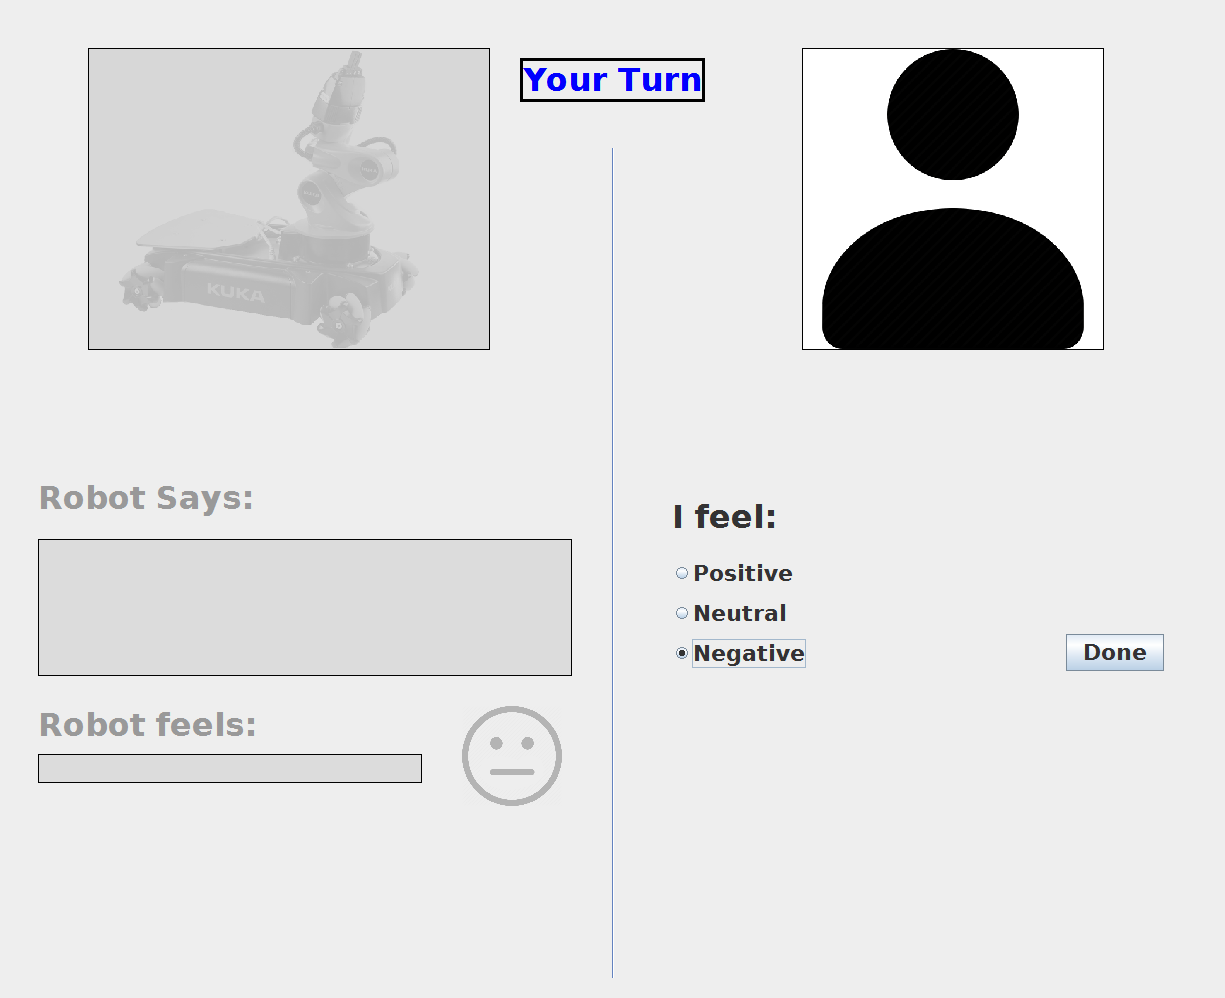
\includegraphics[width=.95\linewidth]{figure/human-turn-gui.png}
  \label{fig:gui-human}
\end{subfigure}
\caption{\fontsize{10}{10}\selectfont The Graphical User Interface (GUI) used
during interaction.}
\label{fig:gui}
\end{figure}

\subsection{Interaction Paradigms}
\label{sec-interaction-paradigms}
At the beginning of each collaboration the robot asked each participant to
achieve the overall shared goal, i.e., ``installing the solar panel''. Then,
before working towards a new goal, the robot informed the participant about the
higher level nonprimitive goal (e.g. Prepare Panel -- see Figure
\ref{fig:collaboration_structure}) of which the primitives were going to be
working towards. The same procedure was used by the robot if there was a
decision to switch to another nonprimitive due to the failure of a task in
achieving the current goal. After achieving a new primitive goal, the robot
either informed the human that it would pursue the next goal, or it informed and
passed the turn to the human to execute the next task with respect to the
human's goal. In case of the human's turn, the robot waited for the human to do
a task, then the wizard let the robot know whether the human's goal was achieved
or not. Afterwards the robot made a decision about which goal to pursue and
informed the human accordingly. The same procedure was applied to both
conditions.

The robot interacted via a) speech, b) the corresponding utterance on the
screen, c) negative, positive and neutral expression of emotion through an
emoticon on the screen. There were two conditions of the robot: 1)
emotion-aware and 2) emotion ignorant. The robot used neutral expression in the
case of emotion-ignorance. The interaction was controlled autonomously by the
framework we discussed in Section \ref{sec:theory} in both the emotion-ignorant
and the emotion-aware cases. The reasoning about which task should be done and
controlling the robot was entirely autonomous. Only the perception of the task
failure or achievement by the robot or by the participant was done by a wizard
monitoring the collaboration outside of the test area. The interaction was
structured based on the exact same goals in the same HTN for both conditions.
The robot was using the same utterances in both conditions. In the emotion-aware
condition the robot used a different behavior in comparison with the
emotion-ignorant condition only if the participant was expressing a negative
emotion in the event of a failure; i.e., the robot's utterances were identical
in emotion-ignorant and emotion-aware cases if in the latter the participant
reported (expressed) a positive or a neutral emotion.

Three different behaviors could be generated only in the emotion-aware
condition. These three behaviors were 1) mitigating the human's negative emotion
and postponing its own task to help the human, 2) goal-management to switch to
another goal which has lower cost with respect to the human's negative emotion,
and 3) task delegation to the human to overcome the impasse. In each run, the
human had two pre-coordinated task failures, and the robot had one. If the human
expressed negative emotion after the first human task-failure, the robot
responded by mitigating the human's negative emotion by saying  ``It was not
your fault. I can help you with this task" and helping the human by providing a
peg to fulfill the human's task. If the human expressed negative emotion after
the second human task-failure, the robot informed the human that they could
proceed with another task to save time while simultaneously requesting a new peg
(i.e. help) from the supervisor. If the human expressed negative emotion as a
result of the robot's task failure, the robot requested help from the human (who
had the correct peg). In the event that the human expressed positive or neutral
emotion during these three failures, the robot behaved identically in the
emotion-ignorant and the emotion-aware cases, by asking the supervisor for help. 

\subsection{Environment and Tasks}

The environment was set up in the Human-Robot Interaction lab and included the
robot, the collaboration board on top of a desk, and the participant standing in
front of the robot on the other side of the board (see Figure
\ref{fig:environment}). One of the experimenters monitored the interactions
using a live stream of a camera in a different room. The experimenter provided
only the required perception, i.e., decision on success or failure of the tasks
for the robot, through the entire time of the collaboration (see Section
\ref{sec-interaction-paradigms}).

The tasks were defined based on the HTN structure shown in Figure
\ref{fig:collaboration_structure} and were executed in a turn-taking fashion by
either of the collaborators. For each task either the robot or the participant
was responsible to pick up one of the corresponding pegs from their own
inventory and place it on the right spot which was colored and tagged the same
as the associated peg. Some pegs and corresponding spots on the board had hidden
magnets which prevented the pegs from standing upright. Any peg that fell over
was considered a failed task.

\section{Evaluation}
\subsection{Hypothesis}

The non/social functions of emotions impact a collaboration process. Human
collaborators prefer to collaborate with others whose behaviors are influenced
by these functions of emotions depending on the context. We developed seven
hypotheses on positive influence of emotion-awareness and usefulness of emotion
function during collaboration:

\textit{\textbf{Hypothesis 1.}} Participants will feel closer to the emotion-aware
robot rather than the emotion-ignorant robot.

\textit{\textbf{Hypothesis 2.}} Participants will find the emotion-aware robot to be
more trustworthy than the emotion-ignorant robot.

\textit{\textbf{Hypothesis 3.}} Participants will find the emotion-aware robot to
have better performance in collaboration than the emotion-ignorant robot.

\textit{\textbf{Hypothesis 4.}} Participants will find the emotion-aware robot to be
more understanding of their feelings than the emotion-ignorant robot.

\textit{\textbf{Hypothesis 5.}} Participants will find the emotion-aware robot to be
more understanding of their goals than the emotion-ignorant robot.

\textit{\textbf{Hypothesis 6.}} Participants will feel more satisfied about the
collaboration when working with the emotion-aware robot rather than
emotion-ignorant robot.

\textit{\textbf{Hypothesis 7.}} Participants will perceive higher level of mutual
satisfaction with the emotion-aware robot than emotion-ignorant robot.

\begin{figure}
  \centering
  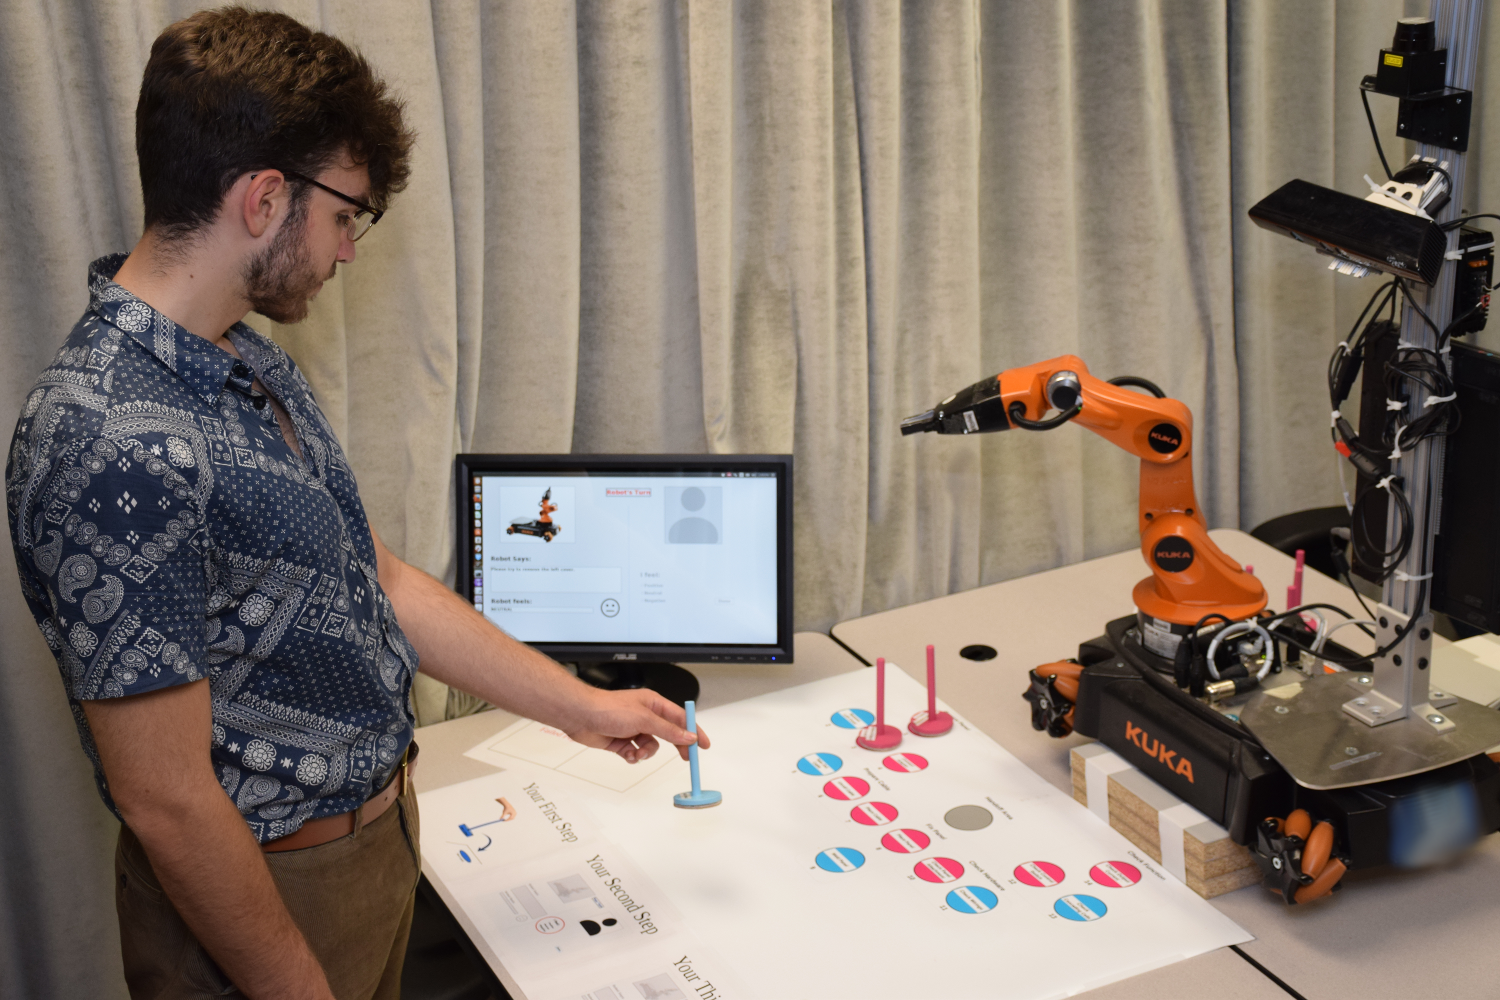
\includegraphics[width=0.9\textwidth]{figure/environment.png}
  \caption{\fontsize{10}{10}\selectfont Experimental setup.}
  \label{fig:environment}
\end{figure}

\subsection{Procedure}
\label{sec:procedure}
Participants were first given a brief description of the purpose of the
experiment. After the short introduction, they were asked to review and sign a
consent form. Participants were then provided with a written instruction of
their task and the rules for collaborating with the robot. Then, one of the
experimenters lead them into the experiment room and asked the participants
to asked to answer pre-experiment questionnaires. Afterwards, the experimenter
went through all the details of the instructions with the participants
standing in front of the collaboration board and the robot. The experimenter
confirmed participants' correct understanding of the tasks and informed them
of types of task failures that might occur during the collaboration.
Participants were told that researchers were developing a collaborative robot
and would like their help in evaluating their design. Participants were provided
with identical instructions and randomly assigned to complete either the
emotion-aware or the emotion ignorant condition first. They were told that,
after their collaboration with the robot, they would be asked to answer a
questionnaire on their experience. After completing the first round of
collaboration, participants answered a post-experiment questionnaire that
measured their perceptions of the robot, the task, and the collaboration
procedure. After answering the first post-experiment questionnaire, participants
were told that they were going to collaborate with the robot one more time and
the robot might not necessarily have the same collaborative behavior. After
completing the second round of collaboration, participants were asked to answer
the second post-experiment questionnaire which consisted of the same questions
as the first post-experiment questionnaire. After all, participants were asked
to answer an open-ended questionnaire which measured their perception of
difference between two runs, their preference of collaborative robot between two
runs, and their reasons of preference.

\subsection{Measurements}
\label{sec:Measurements}
In our study two basic conditions of the robot were tested: a) the
emotion-ignorant condition, b) the emotion-aware condition. We measured
participants' recall of the collaborative behaviors presented by the robot using
an open-ended post-experiment questionnaire. We also specifically asked the
participants what behavior of the robot they liked during their collaboration.
We also evaluated participants' levels of satisfaction, trust, goal achievement,
mutual understanding of goals, mutual understanding of feelings, mutual
agreement, and also participants' beliefs about the efficiency of collaboration
and their feeling of robot's collaborative behaviors. Seven-point Likert scales
were used in these questionnaire items.

\subsection{Participants}
\label{sec:Participants}
A total of 37 participants participated in the experiment in 74 trials.
Participants were recruited from Worcester Polytechnic Institute's students and
staffs as well as other civilians recruited from outside of the campus. The ages
of the participants varied between 19 and 74 with an average of 34.2 years
before our screening of 4 participants based on our sanity check questions. After
this screening the ages of the participants varied between 19 and 54 with an
average of 30.8 years old. Of the 33 participants, 21 were female and 12
were male. Each participant participated in 2 trials. In one trial the robot was
aware of human's emotion and in the second trial the robot was ignoring human's
emotion. The order of these two trials were randomly assigned to each
participant. In general we used emotion-ignorant robot first in 16 experiments,
and emotion-aware robot first in 17 experiments.

\section{Results}

As discussed in Section \ref{sec:Measurements}, results of the user study were
gathered through a 31-question Likert-scale survey that was given to each
participant after each run with the robot, and through a 5-question open-ended
summary questionnaire at the end of the experiment.

\begin{figure*}[h]
\centering
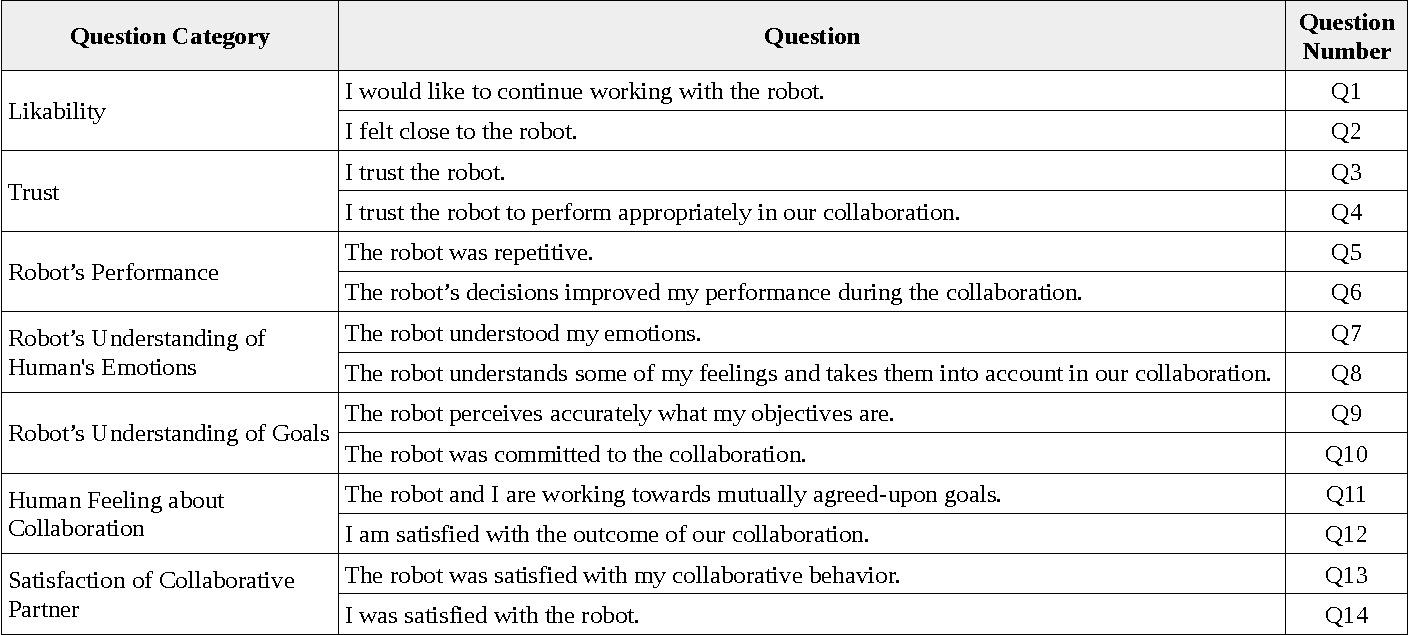
\includegraphics[width=0.81\textwidth]{figure/table1-croped.pdf}
\caption{\fontsize{10pt}{10pt}\selectfont The 31 Likert scale questions
organized according to their groups.}
\label{fig:31questions-table}
\end{figure*}

\subsection{7-Point Likert Scale Survey Results}
As mentioned previously, the 7-point Likert scale survey was administered at
the end of the emotion-ignorant run and at the end of the emotion-aware run for
each participant. The 31 questions are generally categorized to evaluate the
humans' perceptions of the following seven categories, with 3-7 questions per
group: (1) the likability of the robot (2) the level of trust the human feels
in the robot (3) the human's perception of the robot's performance (4) the
human's perception of the robot's understanding of human's emotions (5) the
human's perception of the robot's understanding of human's and collaboration's
goals and objectives (6) the human's feeling about the collaboration and (7)
the human's perception of the human's and robot's mutual satisfaction with each
other as collaborative partners. The questions presented are provided in Figure
\ref{fig:31questions-table}.

The results were analyzed using a two-tailed paired t-test to analyze the
difference of means between the emotion ignorant and the emotion-aware
condition. Refer to Figures \ref{fig:overall-performance} -
\ref{fig:overall-satisfaction} for the results. As mentioned in Section
\ref{sec:Participants}, participants were randomly assigned to complete either
the emotion-ignorant or the emotion-aware run first; analysis of the results
revealed no statistically significant difference or consistent pattern based on
which run the participant completed first.

\vspace*{-5mm}
\begin{figure*}
 \centering
 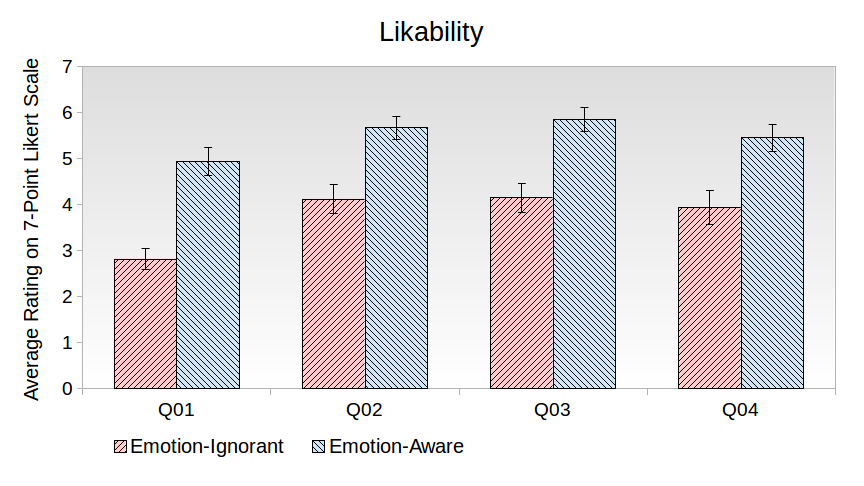
\includegraphics[width=0.8\textwidth]{figure/Overall-Likability.png}
 \vspace*{-5mm}
 \caption{\fontsize{10}{10}\selectfont Results of the Likert scale survey for
 Likability questions. The p-value for the difference between means is
 $\ll$0.001 for all questions.}
 \label{fig:overall-likability}
 \vspace*{-5mm}
\end{figure*}

\subsubsection{Likability of the Robot}
\label{sec:Likability}
Questions 1 through 4 addressed the likability of the robot. As shown in Figure
\ref{fig:overall-likability}, participants rated the emotion-aware robot
1.5-2.1 points higher than the emotion-ignorant robot. These results
indicate that participants felt closer with and preferred working with the
emotion-aware robot; these results support Hypothesis 1, which stated that
humans would prefer to work with the emotion-aware robot over the
emotion-ignorant robot.

\subsubsection{Human Trust in the Robot}
\label{sec:Trust}
Questions 5-9 were designed to measure the degree of trust that the human
participants felt in the robot. As shown in Figure \ref{fig:overall-trust},
participants trusted the emotion-aware robot, on average, a minimum of 1.4
points more than the emotion-ignorant robot, both in general and in terms of
collaboration performance. In Question 5, participants rated a
general statement of trust 1.5 points higher in the emotion-aware
case. Additionally, in Question 7, participants rated their trust in the
emotion-aware robot to perform appropriately during collaboration an average of
5.9 on a 7-point Likert scale, where 7.0 would indicate maximum trust; this
indicates an acceptable level of trust in the robot's collaborative
abilities. These results support Hypothesis 2, that posits that human
participants would find the emotion-aware robot to be more trustworthy than the
emotion-ignorant robot.

\vspace*{-5mm}
\begin{figure*}[tbh]
\centering
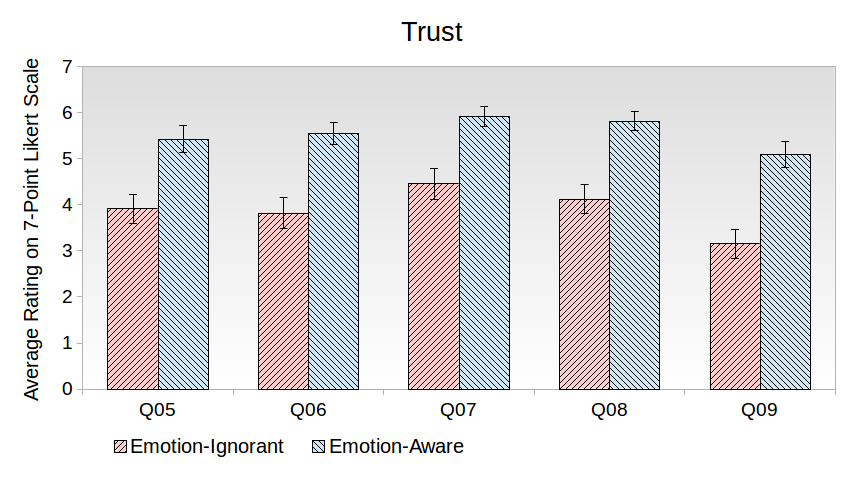
\includegraphics[width=0.8\textwidth]{figure/Overall-Trust.png}
\vspace*{-5mm}
\caption{\fontsize{10}{10}\selectfont Results of the Likert scale survey for
questions related to trust. The p-value for the difference between means is
$\ll$0.001 for all questions.}
\label{fig:overall-trust}
\vspace*{-5mm}
\end{figure*}

\begin{figure*}[tbh]
\centering
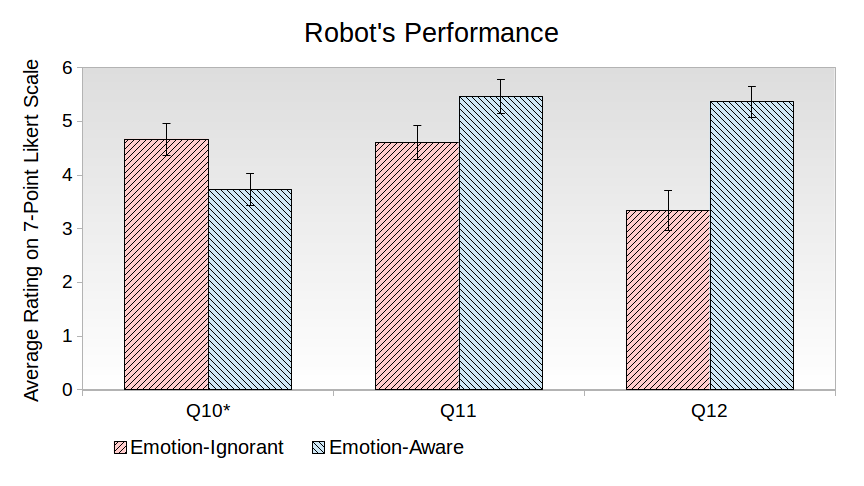
\includegraphics[width=0.8\textwidth]{figure/Overall-Performance.png}
\caption{\fontsize{10}{10}\selectfont Results of the Likert scale survey for
questions related to the robot's performance. The p-value for the difference
between the means for questions 10, 11 and 12 are 0.001, 0.063 and $\ll$0.001,
respectively.}
\label{fig:overall-performance}
\end{figure*}

\subsubsection{Perception of the Robot's Performance} 
\label{sec:Performance}
Question 10 (which is reverse-scored) measures the participant's perception of
repetitiveness in the robot during the collaboration. In both conditions,
participants rated the robot as moderately repetitive, with the emotion-ignorant
robot's average response being about 1.1 points higher than the emotion-aware.
This result correlates with several of the open-ended responses which described
the emotion-aware robot's behaviors as ``cute'' and ``interesting'', refer to
Section \ref{sec:Open-Ended}. Question 11, which asks about the efficiency of
the robot's decisions is the only question of the 31 questions that did not have
a statistically significant difference between the emotion-aware and the
emotion-ignorant case. This correlates with the result of the open-ended
question asking which condition of the robot exhibited behaviors that could
prevent human error (refer to \ref{sec:Open-Ended}); in response to this
question, several respondents stated that it may be quicker or simpler to call
the supervisor in the event of a task failure, rather than changing the order of
the tasks. According to the results from Question 12, the participants felt that
the emotion-aware robot's decisions during collaboration improved their own
performance, with an average rating of 5.4, while the emotion-ignorant robot
only received an average rating of 3.3, indicating that participants felt it was
not able to interact in such a way as to increase the human's performance; refer
to results from Question 6. These results support Hypothesis 3, which posited
that humans will perceive the emotion-aware robot as being more capable than the
emotion-ignorant robot.

\subsubsection{Robot's Understanding of Human Emotions} 
\label{sec:Emotions}
In Questions 13 through 17, participants evaluate the robot's understanding of
humans' emotions. In questions 13, 15, and 16, participants rated the
emotion-aware robot, on average, a minimum of 1.8 points higher than the
emotion-ignorant robot. In response to questions 14 and 17, which are
reverse-scored, participants ranked the emotion-ignorant robot 1.2 and 2.0
points higher, respectively, than then emotion-aware robot. The results
of all five questions in this category support Hypothesis 4.

\vspace*{-5mm}
\begin{figure*}[tbh]
\centering
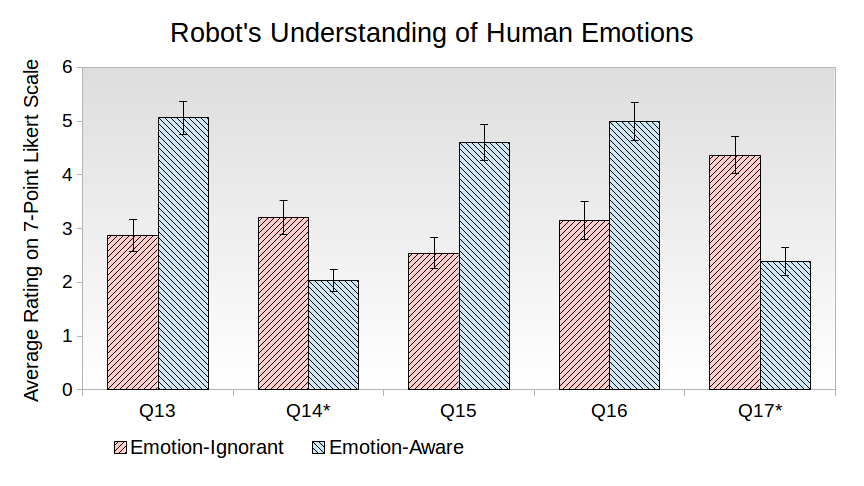
\includegraphics[width=0.8\textwidth]{figure/Overall-Emotions.png}
\vspace*{-5mm}
\caption{\fontsize{10}{10}\selectfont Results of the Likert scale survey for the
questions related to the robot's understanding of human emotions. The p-value
for the difference between the means is $\ll$0.001 for all of the questions
except Question 14, for which the p-value is 0.003.}
\label{fig:overall-emotions}
\vspace*{-5mm}
\end{figure*}

\subsubsection{Robot's Understanding of Human and Collaboration Goals}
\label{sec:Goals}
Questions 18 and 19 were reverse-scored questions intended to determine whether
the humans felt that the robot understood the shared collaboration goal and the
human's personal goal, respectively. For both conditions of the robot, the
average scores were lower than 3.5, indicating that the human's perceived the
robot as having some understanding of the goals. For both questions, the
emotion-ignorant robot's average score was significantly higher than the
emotion-aware robot's score. Similarly, Question 20 was a measure of whether the
human perceived that the robot correctly perceived the human's goal.
On average, participants provided an average rating for the emotion-aware robot
that was 1.5 points higher than that for the emotion-ignorant robot. Question 21
measured the human perception of the robot's commitment to the collaboration;
for this measure, the average participant score assigned to the emotion-aware
robot was 6.2 points out of a maximum of 7 points, indicating that the
participants felt that the emotion-aware robot was strongly committed to the
collaboration. The emotion-ignorant robot received an average rating of 4.4
points, indicating only moderate commitment. These results strongly support
Hypothesis 5, which posits that humans will feel that the emotion-aware robot
will better understand their goals than the emotion-ignorant robot.

\begin{figure*}
\centering
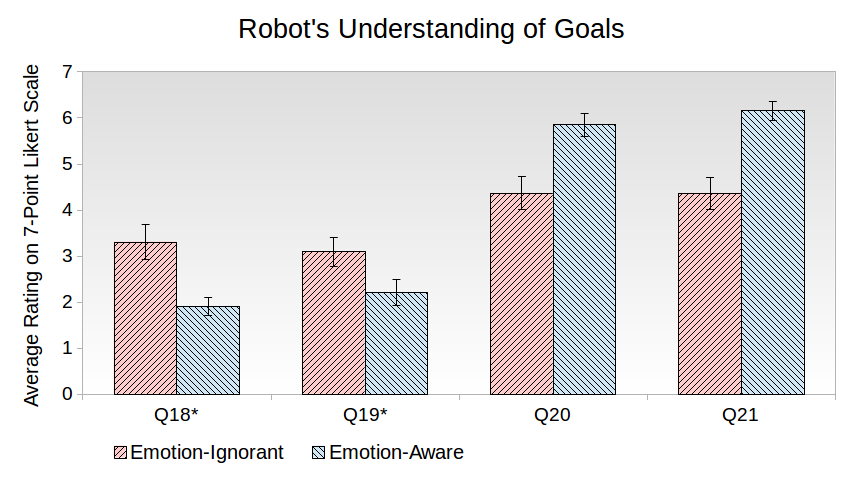
\includegraphics[width=0.8\textwidth]{figure/Overall-Goals.png}
\caption{\fontsize{10}{10}\selectfont Results of the Likert scale survey for
questions related to the robot's understanding of goals. The p-value for the
difference between the means for all questions is $\ll$0.001, except Question
19, for which the p-value is 0.006.}
\label{fig:overall-goals}
\end{figure*}

\begin{figure*}
\centering
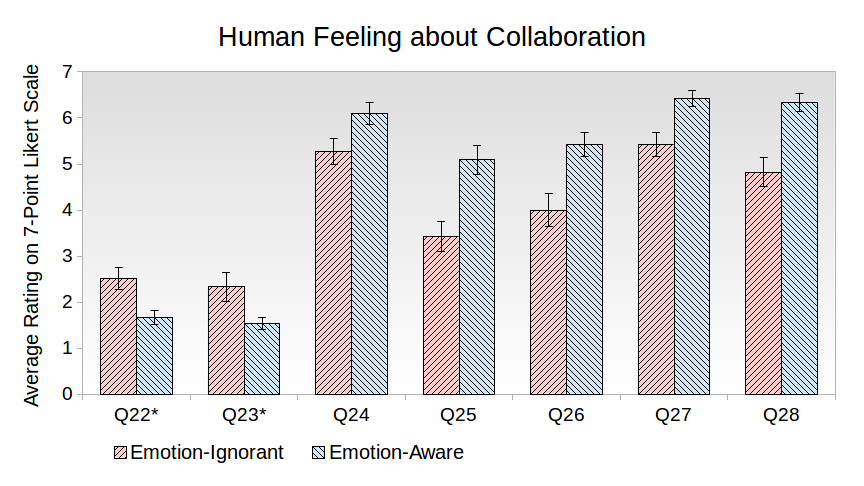
\includegraphics[width=0.8\textwidth]{figure/Overall-Collaboration.png}
\caption{\fontsize{10}{10}\selectfont Results of the Likert scale survey for
questions related to the human's feeling about the collaboration. The p-value
for the difference between the means is $\ll$0.001 for questions 22, 25, 26, and
28. The p-value for Questions 23, 24 and 27 are 0.02, 0.008 and 0.001,
respectively.}
\label{fig:overall-collaboration}
\end{figure*}

\subsubsection{Human's Feeling about the Collaboration}
\label{sec:Collaboration}
Questions 22 through 28 were designed to gauge how the human participants
felt about the partnership within the collaboration and the outcome of the
collaboration. For each of the 7 questions, the participants ranked the
emotion-aware robot as better than the emotion-ignorant robot, by a minimum,
on average, of 0.8 points. Questions 24, 27 and 28 addressed whether the robot
and the participant were working toward mutually agreed-upon goals and on the
outcome of the collaboration; in the emotion-aware condition, participants rated
the robot a minimum of 6.1 points, on average, while rating the emotion-ignorant
robot 1-1.6 points lower, indicating that the participants felt a very strong
sense of collaboration with the emotion-aware robot, and only a moderate sense
of collaboration with the emotion-ignorant robot. Questions 25 and 26 address
whether the robot and the participant set the collaboration goals together;
these two questions have lower scores than Questions 24, 27 and 28, for both the
emotion-aware and the emotion-ignorant case. The lower overall scores are
likely due to the fact that the robot decides the task order or action in the
event of failure in both conditions; however, the higher score in the
emotion-aware case may indicate that emotional awareness can increase a feeling
of collaboration. These results support Hypothesis 6 that humans will feel
a greater sense of mutual collaboration and understanding about the
collaboration with the emotion-aware robot.

\subsubsection{Human Perception of Mutual Satisfaction with Collaborative
Partner}
\label{sec:MutualSatisfaction}
Questions 29, 30 and 31 were designed to measure the human's perception
of the robot's satisfaction with the human, the human's satisfaction with the
robot and the mutual understanding between the human and the robot,
respectively. The participants provided an average response in the emotion-aware
condition of 5.8, 5.9 and 5.7 to Questions 29, 30 and 31, respectively,
indicating a high level of mutual satisfaction; all three answers were
about 1.4-1.9 points lower, on average, in the emotion-ignorant condition. These
results indicate a higher level of satisfaction working with the robot in the
emotion-aware condition, and strongly support Hypothesis 7, which posited that
humans will feel a greater sense of mutual satisfaction with the emotion-aware
robot than the emotion-ignorant robot.

\begin{figure*}
\centering
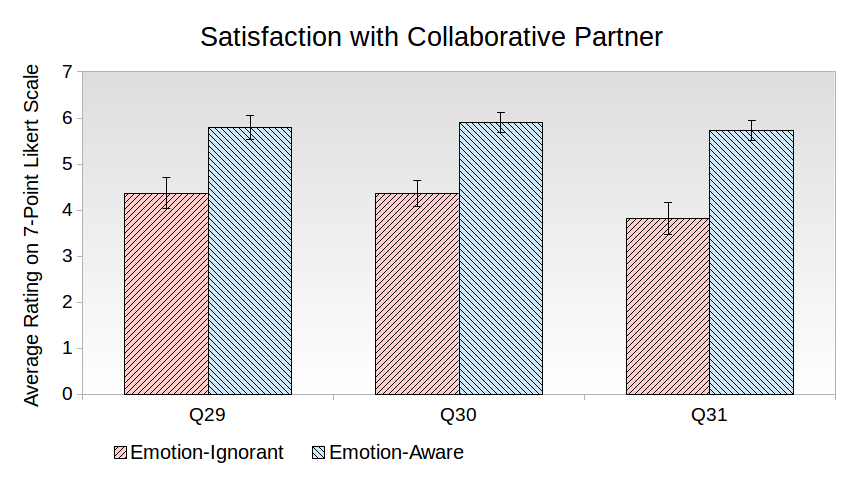
\includegraphics[width=0.8\textwidth]{figure/Overall-Satisfaction.png}
\caption{\fontsize{10}{10}\selectfont Results of the Likert scale survey for
questions related to satisfaction with collaborative partner. The p-value for
the difference between means is $\ll$0.001 for all questions.}
\label{fig:overall-satisfaction}
\end{figure*}

\subsection{Results from the Open-Ended Questionnaire} 
\label{sec:Open-Ended}
As described in Section \ref{sec:procedure}, each participant answered an open-ended
questionnaire at the end of the study. Figure \ref{fig:Open-Ended-Table}
summarizes the questionnaire and which run users preferred for certain
conditions (i.e. emotion-ignorant or emotion-aware). Note that some users chose
not to state a preference regarding which run they preferred for certain
conditions; because we were specifically interested in whether users preferred
the emotion-aware case, we considered the ambiguous responses to be failures in
the binomial analysis. The binomial analysis is based off of a population size
of 33. 

\begin{figure*}[tbh]
\centering
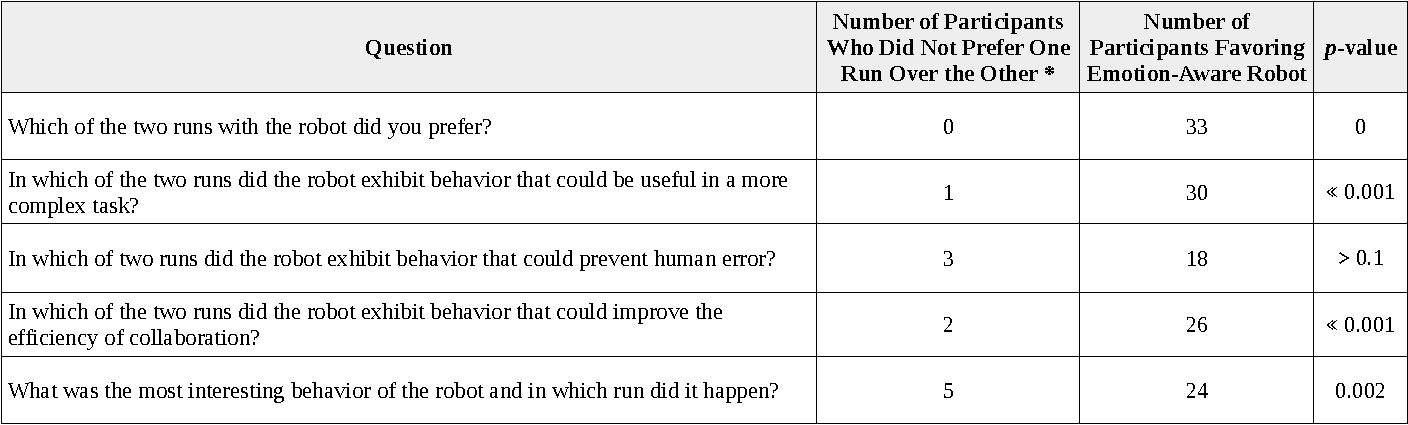
\includegraphics[width=1\textwidth]{figure/table2-croped.pdf}
\caption{\fontsize{10pt}{10pt}\selectfont Open-ended questionnaire questions and
results. (*Note: Because we are evaluating whether humans prefer an
emotion-aware robot, these results are taken as negative test results when
calculating the p-value using the binomial distribution. Only those participants
who clearly indicated a preference for the emotion-aware robot are taken as
positive test results.)}
\label{fig:Open-Ended-Table}
\vspace*{-5mm}
\end{figure*}

As shown in Figure \ref{fig:Open-Ended-Table}, 100\% of users unambiguously
preferred the run with the emotion-aware robot. In general, this preference
stemmed from a feeling of closeness and partnership, as seen in these responses:
``the robot had emotions and responded to my emotions. Also, what it said about
my failing was cute and aimed to make me feel better.'' Another example is ``I
liked feeling needed and accounted for; I felt closer to the robot.'' Finally,
``I saw the changes in its feeling, which motivated me to care more about my
act...I also liked that he asked me to correct its failure, although it could
ask the supervisor.''  

When asked in which of the two runs the robot exhibited
behavior that could be useful in a more complex task, 90.9\% chose the
emotion-aware robot. In general, respondents thought that the emotion-aware
robot was better at problem solving, more adaptable, and more capable of
handling the social complexities that occur in collaboration, as shown in
responses such as ``The robot explained motives...which is important to keep a
team communicating and on the same pace.'' Also, ``When we failed he initially
switched to a new task and then came back to the originally failed task. It kept
me from getting irritated and negative.'' Finally, ``The more complex, the more
necessary it is to understand how humans think and operate...an empathetic robot
can adapt, encourage and help.'' It is worth noting that one respondent
preferred the emotion-ignorant case, saying ``In a more complex task it might be
better for the robot to take control and simply tell me what to do; trying to be
understanding and collaborative wouldn't be as important as doing the task
correctly.''

The only question that did not provide statistically significant support in
favor of the emotion-aware robot related to which case the robot exhibited
behavior that could prevent human error. About 36.4\% of respondents thought
that the emotion-ignorant robot was more likely to prevent human error; however, all
but one of these cited calling the supervisor as the main method of preventing
human error, in spite of the fact that the instructions indicated that the
robot's need to call the supervisor counted against the collaboration. Of the
54.5\% who thought that the emotion-aware robot was better at preventing human
error, most cited the robot's ability to console the human as the main behavior
that could prevent human error. Respondents indicated that this enabled them to
move on and feel better about the collaboration, as with this response: ``The
robot switched to a different task and we came back to an error later. This
allowed my mind to move away from being frustrated. I was able to complete a
different task which felt like a win - then come back and finish the error.
Making my mind move away from frustration could definitely prevent more
errors.''

When asked in which of the runs the robot exhibited behavior that could improve
the efficiency of the collaboration, 78.8\% responded with the emotion-aware
case; of these, the vast majority stated that this was because of the robot's
ability to change the order of tasks in the event of a failure, and to ask the
human for help.

Finally, when asked in which run the most interesting behavior occurred,
72.7\% chose the emotion-aware condition. Of these respondents, 12
individuals stated that the robot's attempt to console the human by saying ``It
was not your fault'' in response to the human's negative emotion that occurred
as a consequence of the human's failed task was the most interesting behavior,
and a majority mentioned that it actually made them feel more positive. Six
participants referred to the robot's ability to understand and express emotion.
Several participants referred to the robot's ability to communicate, including
the ability to ask questions. Of those who responded with the emotion-ignorant
case, most found the ability to call the supervisor, and mechanical functions,
such as gripping, to be most interesting.

\subsection{Impact of Demographics} 
As mentioned in Section \ref{sec:Participants}, we recorded certain demographic
information from each participant, including age and gender. We also had each
participant complete several personality questionnaires. Although it was not the
primary purpose of the study, we investigated the Likert scale results to
determine if there were any relevant trends based on the demographics and
personalities of the participants. A close study of the results did  not reveal
any identifiable pattern based on gender or personality.

\begin{figure*}[tbh]
\centering
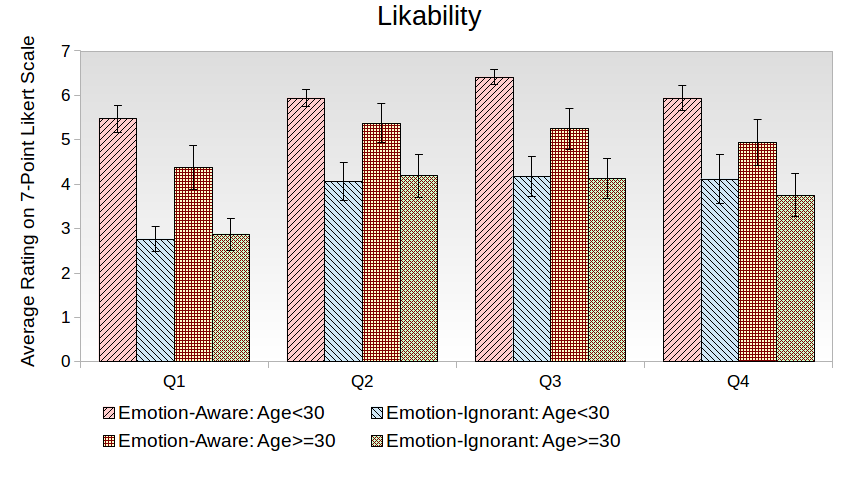
\includegraphics[width=0.9\textwidth]{figure/Age-Likability.png}
\vspace*{-5mm}
\caption{\fontsize{10pt}{10pt}\selectfont Impact of age on results of Likert
scale questions related to likability.}
\label{fig:age-likability}
\end{figure*}

Age did reveal an interesting pattern. We divided the participants into two
groups, below 30 years of age and 30 or above. While question-by-question
comparisons revealed only a few statistically significant differences based on
age, a general pattern emerged. For all but four of the 31 questions presented,
the younger age group reported higher scores than the older age group (or lower,
in the case of reverse-scored questions)for the emotion-aware robot. In the
emotion-ignorant case, the younger group tends to score the robot nearer to
the same value as the older age group for all but seven questions, leading to a
pattern in which the score drop between the emotion-aware and the
emotion-ignorant case was more for the younger group than for the older group;
the seven questions that broke this pattern were 7, 9, 11, 12, 18, 19 and 22.

\begin{figure*}[!h]
\centering
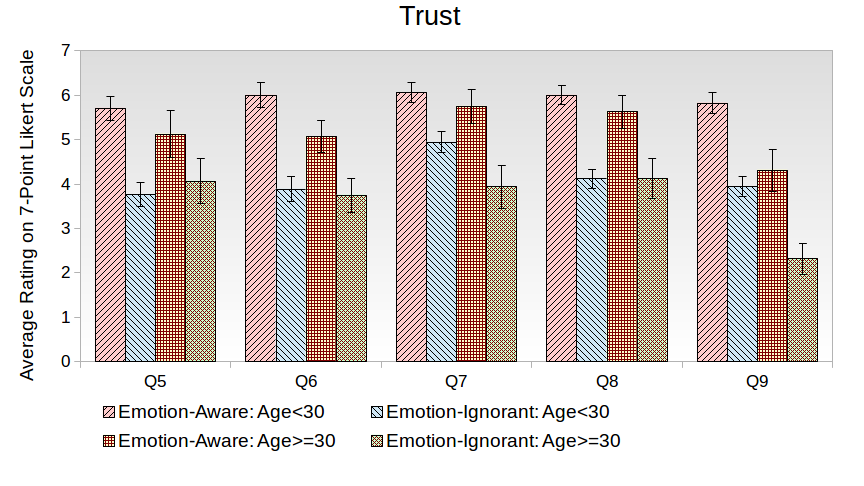
\includegraphics[width=0.9\textwidth]{figure/Age-Trust.png}
\caption{\fontsize{10pt}{10pt}\selectfont Impact of age on results of Likert
scale questions related to trust.}
\label{fig:age-trust}
\end{figure*}

\begin{figure*}[!h]
\centering
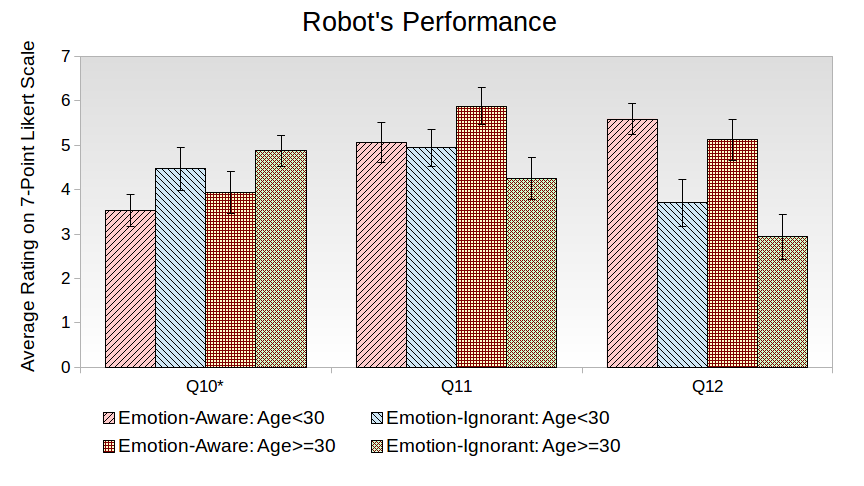
\includegraphics[width=0.9\textwidth]{figure/Age-Performance.png}
\caption{\fontsize{10pt}{10pt}\selectfont Impact of age on results of Likert
scale questions related to performance.}
\label{fig:age-performance}
\vspace*{15mm}
\end{figure*}

\begin{figure*}[!h]
\centering
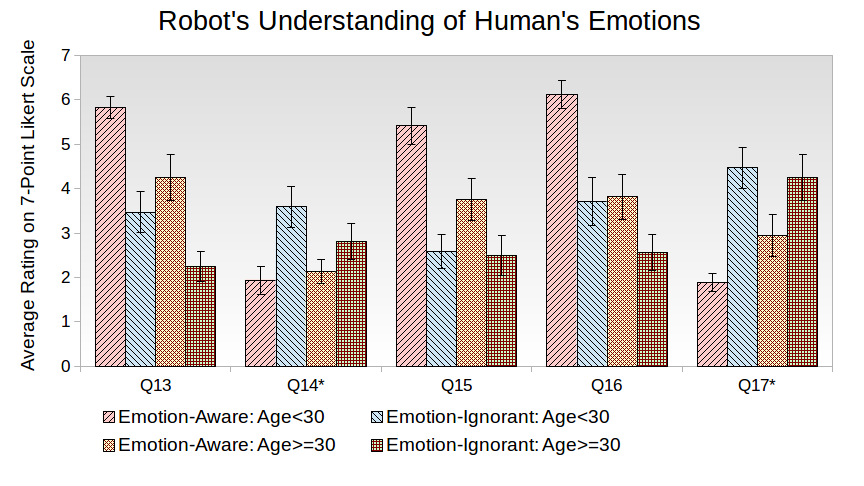
\includegraphics[width=0.9\textwidth]{figure/Age-Emotions.png}
\caption{\fontsize{10pt}{10pt}\selectfont Impact of age on results of Likert
scale questions related to robot's understanding of human's emotions.}
\label{fig:age-emotions}
\vspace*{15mm}
\end{figure*}

\begin{figure*}[!h]
\centering
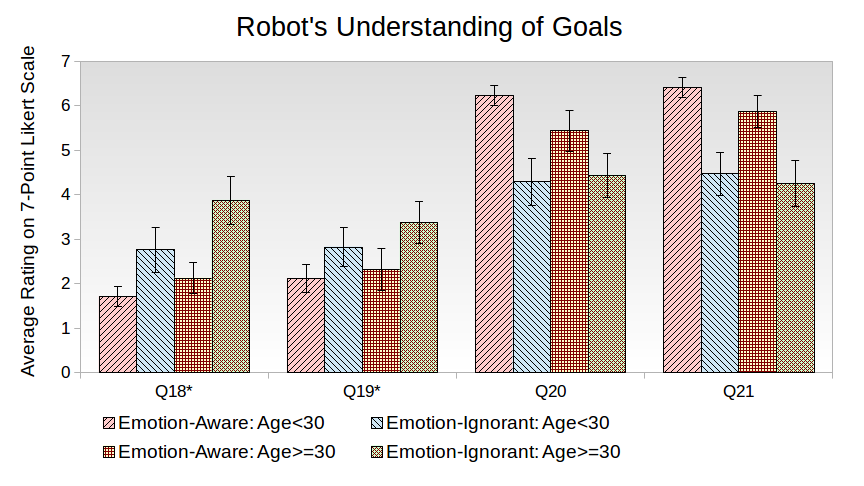
\includegraphics[width=0.9\textwidth]{figure/Age-Goals.png}
\caption{\fontsize{10pt}{10pt}\selectfont Impact of age on results of Likert
scale questions related to robot's understanding of goals.}
\label{fig:age-goals}
\vspace*{10mm}
\end{figure*}

\begin{figure*}[!h]
\centering
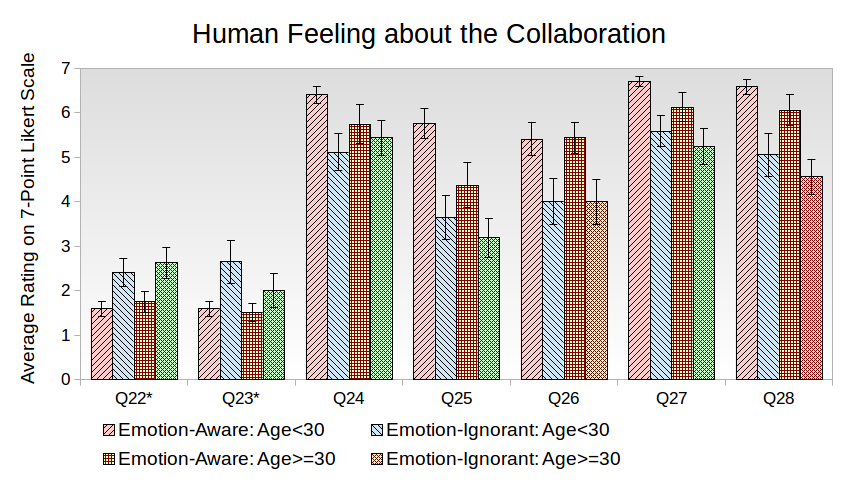
\includegraphics[width=0.9\textwidth]{figure/Age-Collaboration.png}
\caption{\fontsize{10pt}{10pt}\selectfont Impact of age on results of Likert
scale questions related to human's feeling about collaboration.}
\label{fig:age-collaboration}
\vspace*{15mm}
\end{figure*}

\begin{figure*}[!h]
\centering
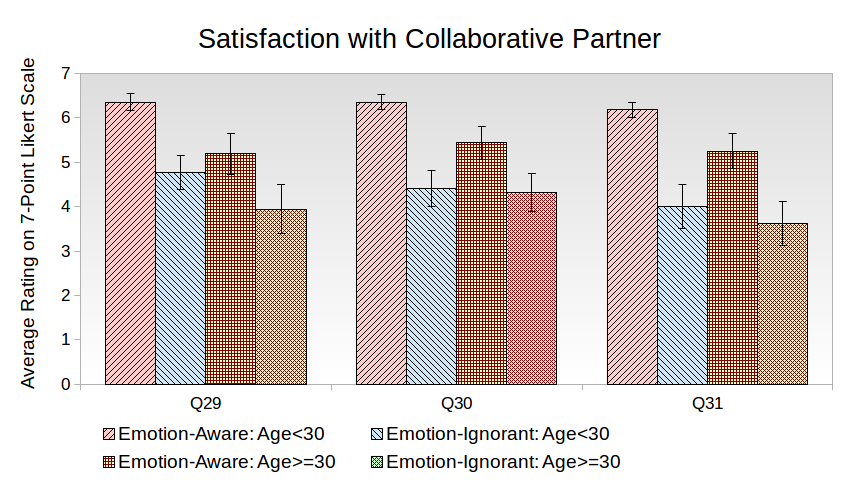
\includegraphics[width=0.9\textwidth]{figure/Age-Satisfaction.png}
\caption{\fontsize{10pt}{10pt}\selectfont Impact of age on results of Likert
scale questions related to satisfaction with collaborative partner.}
\label{fig:age-satisfaction}
\end{figure*}

\section{Discussion}
Based on the results, all participants prefer to work with the emotion-aware
robot. Humans find the emotion-aware robot more likable and more trustworthy, as
indicated in the Likert-scale responses and the open-ended questionnaire
responses. Based on the responses, the emotional interaction with the robot can
help create a sense of closeness and enjoyment that makes humans want to
continue working with the robot.

The results also indicate that the emotion aware robot can better maintain a
collaborative relationship. Both Likert-scale responses and Open-Ended
Questionnaire responses indicate this. Humans felt a stronger sense of the
robot's commitment to the collaboration, and greater understanding of their
goals and emotions from the robot. Several open-ended responses also indicated
that the robot was able to successfully motivate people and maintain their
commitment to the collaboration, especially when tasks failed. Additionally, as
shown in Section \ref{sec:Performance}, humans rated the emotion-aware case much
higher than the emotion-ignorant case when asked which robot's decisions
improved their performance, in essence acknowledging that their collaborator's
(i.e. the robot's) decisions had a significant impact on their performance. As
some of the open-ended responses indicated, successfully managing emotions
within the collaboration can help keep the collaboration on track, and prevent
distractions due to guilt and other negative emotions.

Finally, the emotion-aware robot developed a stronger sense of  partnership
through greater communication. The participants felt better understood by the
emotion-aware robot, and felt that the goals were more mutually agreed-upon,
refer to Section \ref{sec:Collaboration}. As evidenced in the following
response, the emotion-aware robot was successfully able to create a sense of
partnership through its more open communication style: ``Communication is very
important. In the first run (i.e. emotion-aware) the robot states what tasks he
is working on, it is clear and straight-forward. Also during the first run the
robot cares about the human(me)'s feelings and cheers me up when I failed at the
tasks, I think that could also improve efficiency of collaboration, because it
would be more like a team or partnership.''

\chapter{Conclusion}
\label{ch:conclusion}

\section{Discussion}

\section{Future Work}

\pagebreak

\bibliographystyle{abbrv}
\bibliography{mshayganfar}


\begin{appendices}
\chapter*{Appendix A}
\label{apdx:constraints}
\addcontentsline{toc}{chapter}{A}

\end{appendices}

\end{document}